\chapter{Results}\label{chap:results}

After a survey of the main theoretical CP findings \& modern flavours (Chapter \ref{chap:conformal-prediction}), and the recent workarounds to enable this framework in the non-exchangeable case (Chapter \ref{chap:exchangeability}); this chapter will be devoted to the assessment of two different practical use-cases.

First, in section \ref{sec:implementation} we will briefly review the code implementation in Python and, in section \ref{sec:assessment}, we will discuss how the user can assess several important attributes of the obtained predictive intervals.

Lastly, in section \ref{sec:results-exchangeable} we will present the results of applying CP to a tabular data regression problem; while the non-exchangeable case will be covered in section \ref{sec:results-ts}, in which CP will be applied to a energy demand forecasting problem.

\section{Implementation}\label{sec:implementation}

The code developed for this work can be found at the corresponding author's \href{https://github.com/gcastro-98/conformal-prediction}{repository}. Essentially, the scripts leverage the Python library \href{https://mapie.readthedocs.io/en/stable/index.html#}{\texttt{mapie}}, both for the computation of predictive intervals and the assessment of results.

In particular, regarding the uncertainty quantification procedure, we can distinguish the following Python classes:
\begin{itemize}
    \item \href{https://mapie.readthedocs.io/en/stable/generated/mapie.regression.MapieRegressor.html#mapie.regression.MapieRegressor}{\texttt{mapie.regression.MapieRegressor}}: it deduces valid confidence intervals by evaluating out-of-fold conformity scores on hold-out validation sets. Depending on the different parameters election, one strategy or another can be implemented. In particular, to apply
    \begin{itemize}
        \item SCP:$\ $ \texttt{method$=$"base"} \& \texttt{cv$=$"split"} must be selected.
        \item CV$+$:$\ $ \texttt{method$=$"plus"} \& \texttt{cv$=$K} must be selected, with \texttt{K} the number of cross-validation folds (\textit{e.g.} $10$).
        \item Jackknife's J$+$aB:$\ $ \texttt{method$=$"plus"} \& \texttt{cv$=$Subsample(n\_{}resamplings=n)} must be selected, initializing the \href{https://mapie.readthedocs.io/en/stable/generated/mapie.subsample.Subsample.html#mapie.subsample.Subsample}{\texttt{mapie.subsample.Subsample}} class with a certain \texttt{n} number of bootstrapped resamples (\textit{e.g.} $50$).        
    \end{itemize}
    All the former is implemented in the \href{https://github.com/gcastro-98/conformal-prediction/blob/main/cp/exchangeable.py}{\texttt{cp.exchangeable}} author's module.
    \item \href{https://mapie.readthedocs.io/en/stable/generated/mapie.regression.MapieQuantileRegressor.html#mapie.regression.MapieQuantileRegressor}{\texttt{mapie.regression.MapieQuantileRegressor}}: enables CQR strategy, as proposed by \cite{romano2019}, with the only valid selections: \texttt{method$=$"quantile"} \& \texttt{cv$=$"split"}. The author implements it in the same \href{https://github.com/gcastro-98/conformal-prediction/blob/main/cp/exchangeable.py}{\texttt{cp.exchangeable}} module.
    \item \href{https://mapie.readthedocs.io/en/stable/generated/mapie.regression.MapieTimeSeriesRegressor.html#mapie.regression.MapieTimeSeriesRegressor}{\texttt{mapie.regression.MapieTimeSeriesRegressor}}: enables the conformal prediction framework for single-output time series data by predicting intervals calibrated with out-of-fold residuals. The \texttt{method$=$"enbpi"} implements the EnbPI strategy, as proposed by \cite{chenxu2021a}, which allows you to continuously update conformal scores using the \href{https://mapie.readthedocs.io/en/stable/generated/mapie.regression.MapieTimeSeriesRegressor.html#mapie.regression.MapieTimeSeriesRegressor.partial_fit}{\texttt{partial\_{}fit}} class method. The author leverages this class in the \href{https://github.com/gcastro-98/conformal-prediction/blob/main/cp/ts.py}{\texttt{cp.ts}} module.
\end{itemize}

\section{Assessment}\label{sec:assessment}

When it comes to assessing the benefits of each strategy certain attributes must be taken into account. For instance:
\begin{itemize}
    \item \textbf{Coverage level}: \textit{i.e.} the fraction of true labels which lie within the prediction intervals, with \href{https://mapie.readthedocs.io/en/stable/generated/mapie.metrics.regression_coverage_score_v2.html#mapie.metrics.regression_coverage_score}{\texttt{mapie.metrics.regression\_{}coverage\_{}score\_{}v2}} as metric.
    \item \textbf{Interval width}: the intervals' mean width, which can be turned into score as prescribed by \href{https://mapie.readthedocs.io/en/stable/generated/mapie.metrics.regression_mean_width_score.html} {\texttt{mapie.metrics.regression\_{}mean\_{}width\_{}score}}.
    \item \textbf{"\textit{Informativeness}"}: a trade-off exists between the interval's width (the smaller, the more informative they are) and the statistical coverage. A clear way of assessing this, combining both the $w$ mean width score and the $c$ coverage score, is through the CWC score. 
    
    This metric, implemented by \href{https://mapie.readthedocs.io/en/latest/theoretical_description_metrics.html#coverage-width-based-criterion}{\texttt{mapie.metrics.coverage\_{}width\_{}based}}, was proposed by \cite{khosravi} and is computed as:
    $$ \mathrm{CWC} = (1 - w) * \exp{\left(-\eta (c - (1-\alpha))^2\right)}\ , $$
    where $\eta$ is a balancing term devoted to reward narrow intervals and penalize those that do not achieve a specified coverage probability. 
    \item \textbf{Adaptability}: the ability of achieving (approximate) conditional coverage, measured by the score \href{https://mapie.readthedocs.io/en/stable/generated/mapie.metrics.regression_ssc_score.html#mapie-metrics-regression-ssc-score}{\texttt{mapie.metrics.regression\_{}ssc\_{}score}}. The SSC (Size Stratified Coverage) score computes the maximum violation of the coverage. In particular, the intervals are grouped by width and the coverage is computed for each group. The lower coverage is the maximum coverage violation. An adaptive method is one where this maximum violation is as close as possible to the global coverage. 

    However, it is very important to check that the intervals widths are well spread before drawing conclusions, because this metric is only usable if the predicted intervals have non-constant width.    
    \item \textbf{Computational efficiency}: the amount of computational resources needed to implement each strategy, which could be measured in terms of CPU time (both training and inference).

\end{itemize}
In this work, we use the author's repository \href{https://github.com/gcastro-98/conformal-prediction/blob/main/cp/validate.py}{\texttt{cp.validate}} \& \href{https://github.com/gcastro-98/conformal-prediction/blob/main/cp/visualize.py}{\texttt{cp.visualize}} modules to respectively compute and represent all the former metrics.

\section{Exchangeable data}\label{sec:results-exchangeable}

In this work, we use (through the author's \href{https://github.com/gcastro-98/conformal-prediction/blob/main/cp/data.py}{\texttt{cp.data}} module) the same dataset as the \href{https://mapie.readthedocs.io/en/stable/examples_regression/4-tutorials/plot_cqr_tutorial.html}{\texttt{mapie}'s CQR tutorial} to present the exchangeable data use-case: the \texttt{sklearn} built-in \href{https://scikit-learn.org/stable/modules/generated/sklearn.datasets.fetch_california_housing.html}{California Housing dataset}. 

Chosen in view of being simple and reproducible, in particular no feature engineering is needed; it is composed of 20,640 samples of the following 8 different features:
\begin{itemize}
    \setlength{\itemsep}{0pt}      % space between items
    % \setlength{\parsep}{0pt}        % space between paragraphs
    % \setlength{\baselineskip}{20pt} % space between lines
    \item The median income in block group
    \item The median house age in block group
    \item The average number of rooms per household
    \item The average number of bedrooms per household
    \item The block group population
    \item The average number of household members
    \item The location (latitude \& longitude) of the block group
    \item The label variable: the median house price for a given block group. 
\end{itemize}

The marginal distributions of the dataset are shown in Figure \ref{fig:app-regression-data-distribution} at Appendix \ref{app:regression-problem}, where the complete set of visualizations and plots for the results' analysis can also be found.\\

Due to the dataset complexity and its potential non-linear relationships, a gradient boosting model is chosen as base estimator. In particular, the \texttt{LGBM} regressor is implemented through the library's \href{https://lightgbm.readthedocs.io/en/latest/pythonapi/lightgbm.LGBMRegressor.html#lightgbm.LGBMRegressor}{\texttt{lightgbm.LGBMRegressor}} Python class. 

Furthermore, to automate the hyper-parameters fine-tuning task, a randomized grid-search is implemented using a 5-fold cross-validation. For this particular problem, the found best settings are:
\begin{itemize}
    \setlength{\itemsep}{0pt}
    \item \texttt{learning\_{}rate}: $0.34318$
    \item \texttt{max\_{}depth}: $18$
    \item \texttt{n\_{}estimators}: $75$
    \item \texttt{num\_{}leaves}: $29$
\end{itemize}

Then, 4 strategies are implemented with \texttt{mapie} according to section \ref{sec:implementation} configuration; these are: the Split Conformal Prediction (SCP), the Cross-Validation $+$ (CV$+$), the Jackknife$+$ after Bootstrapping (J$+$aB) and the Conformalized Quantile Regression (CQR).

While all the 4 strategies are able to provide informative prediction intervals, they present differences in their attributes as shown in Table \ref{tab:regression-metrics}. All the code used to generate these results and visualizations can be found at the author's \href{https://github.com/gcastro-98/conformal-prediction/blob/main/regression.ipynb}{regression.ipynb} notebook.

\begin{table}[ht]
\centering

\begin{subtable}{.5\textwidth}
    \hspace{-28mm}
    \begin{tabular}{|c|c|c|c|c|}
    % \hline
    \rowcolor{ColHead}\textcolor{white}{Strategy} & \textcolor{white}{Coverage} & \textcolor{white}{RMSE} & \textcolor{white}{Training time} & \textcolor{white}{Inference time} \\ \hline
    \cellcolor{RowHead}SCP & 0.806 $\pm$ 0.008 & 0.472 $\pm$ 0.007 & 1.602 $\pm$ 0.174 & 0.068 $\pm$ 0.054\\
    \cellcolor{RowHead}CV+ & 0.853 $\pm$ 0.004 & 0.467 $\pm$ 0.009 & 9.329 $\pm$ 2.804 & 7.986 $\pm$ 0.302\\
    \cellcolor{RowHead}J+aB & 0.734 $\pm$ 0.007 & 0.467 $\pm$ 0.009 & 51.210 $\pm$ 5.609 & 9.698 $\pm$ 0.424 \\
    \cellcolor{RowHead}CQR & 0.805 $\pm$ 0.010 & 0.494 $\pm$ 0.013 & 2.601 $\pm$ 0.087 & 0.095 $\pm$ 0.044 \\
    \hline
    \end{tabular}
\caption{Coverage, RMSE, training \& inference times.}
\label{subtab:regression-metrics-1}
\end{subtable}

\begin{subtable}{.5\textwidth}
    \hspace{-28mm}
    \begin{tabular}{|c|c|c|c|c|}
    \rowcolor{ColHead}\textcolor{white}{Strategy} & \textcolor{white}{Coverage} & \textcolor{white}{Width} & \textcolor{white}{CWC} & \textcolor{white}{SSC} \\ \hline
    \cellcolor{RowHead}SCP & 0.806 $\pm$ 0.008 & 0.971 $\pm$ 0.015 & 0.798 $\pm$ 0.004 & --- \\
    \cellcolor{RowHead}CV+ & 0.853 $\pm$ 0.004 & 1.042 $\pm$ 0.005 & 0.784 $\pm$ 0.002 & 0.650 $\pm$ 0.012 \\
    \cellcolor{RowHead}J+aB & 0.734 $\pm$ 0.007 & 0.710 $\pm$ 0.003 & 0.853 $\pm$ 0.001 & --- % 0.390 $\pm$ 0.018 
    \\
    \cellcolor{RowHead}CQR & 0.805 $\pm$ 0.010 & 1.013 $\pm$ 0.013 & 0.790 $\pm$ 0.004 & 0.745 $\pm$ 0.043 \\
    \hline
    \end{tabular}
\caption{Coverage, width, coverage width-based criterion (CWC) score \& size-stratified coverage (SSC) score.}
\label{subtab:regression-metrics-2}
\end{subtable}

\caption{Different strategies' metrics after a 5-fold cross-validation for $\a=0.2$ regression problem.}
\label{tab:regression-metrics}
\end{table}

In particular, some remarks can be drawn:
\begin{itemize}
    \item CQR \&  SCP are those with most statistical efficiency in terms of coverage (the attained "\textit{Coverage}" is closer to the expected $0.80$). 
    \item On the one hand, CQR \& SCP are both based in a 1-fold split of the dataset. Consequently, while their training and prediction times are significantly lower than CV$+$ \& J$+$aB strategies; the predictive power of the base estimator (trained just with $70\%$ of the data) is also slightly lower.
    \item On the other hand, and spite of its large training and inference times, \& J$+$aB offers the best coverage-width ratio (and thus, informative intervals) according to the CWC score. 
    \item Unlike J$+$aB or SCP, CV$+$ \& CQR offers some interval adaptability. In this sense, according to the SSC score, CQR is better not only achieving global coverage but also approximate conditional coverage.
\end{itemize}

In conclusion, CQR seems the best strategy in order to achieve the best marginal and conditional coverage; thus, resulting a specially good choice in those applications needing for a conservative and statistical efficient tool.
The training and inference times constitute good reasons for its election too, but it should be taken into account a large enough dataset is needed for the method to be informative (since the dataset will be split). 

On the contrary, in case predictive power is to be maximized, while minimizing intervals width, and at expenses of some potential coverage loss and almost no adaptability, then J$+$aB should be chosen. Thus, this strategy seems suitable for those applications in which more reckless guesses can be afforded and the highest predictive power with the minimal width is desired.\\

Finally, to provide more in-depth detail about the coverage capabilities of the former strategies, some plots regarding a specific experiment are displayed in Figure \ref{fig:regression-width-coverage}.

In particular, at sub-figures \ref{subfig:regression-width-histograms} \& \ref{subfig:regression-coverage-width}, the ability of CQR \& CV$+$ to adapt the interval width to the situation is displayed opposed to J$+$aB's. Besides, more adaptability is achieved by CQR, because sub-figure \ref{subfig:regression-width-histograms} shows the intervals' width histograms and how CQR features much more variability than CV$+$ (also wider intervals' bins are occupied more frequently). 

Then, sub-figure \ref{subfig:regression-coverage-width} presents the attained coverage in function of the interval widths each strategy yielded, showing how CQR effectively attains more coverage per different width.\\

And lastly, sub-figure \ref{subfig:regression-coverage-alpha} shows the ability to attain global coverage but in function of different $\a$ values (through a 5-fold cross-validation for 5 $\a$ values evenly spaced from $0.20$ to $0.01$). The same conclusions for the $\a=0.2$ analysis apply: CQR \& SCP, and independently of $\a$, are the best when it comes to attaining global coverage.

\begin{figure}[ht]
    \centering
    %\hspace{-10mm}
    \begin{subfigure}[b]{0.32\textwidth}
        \centering
        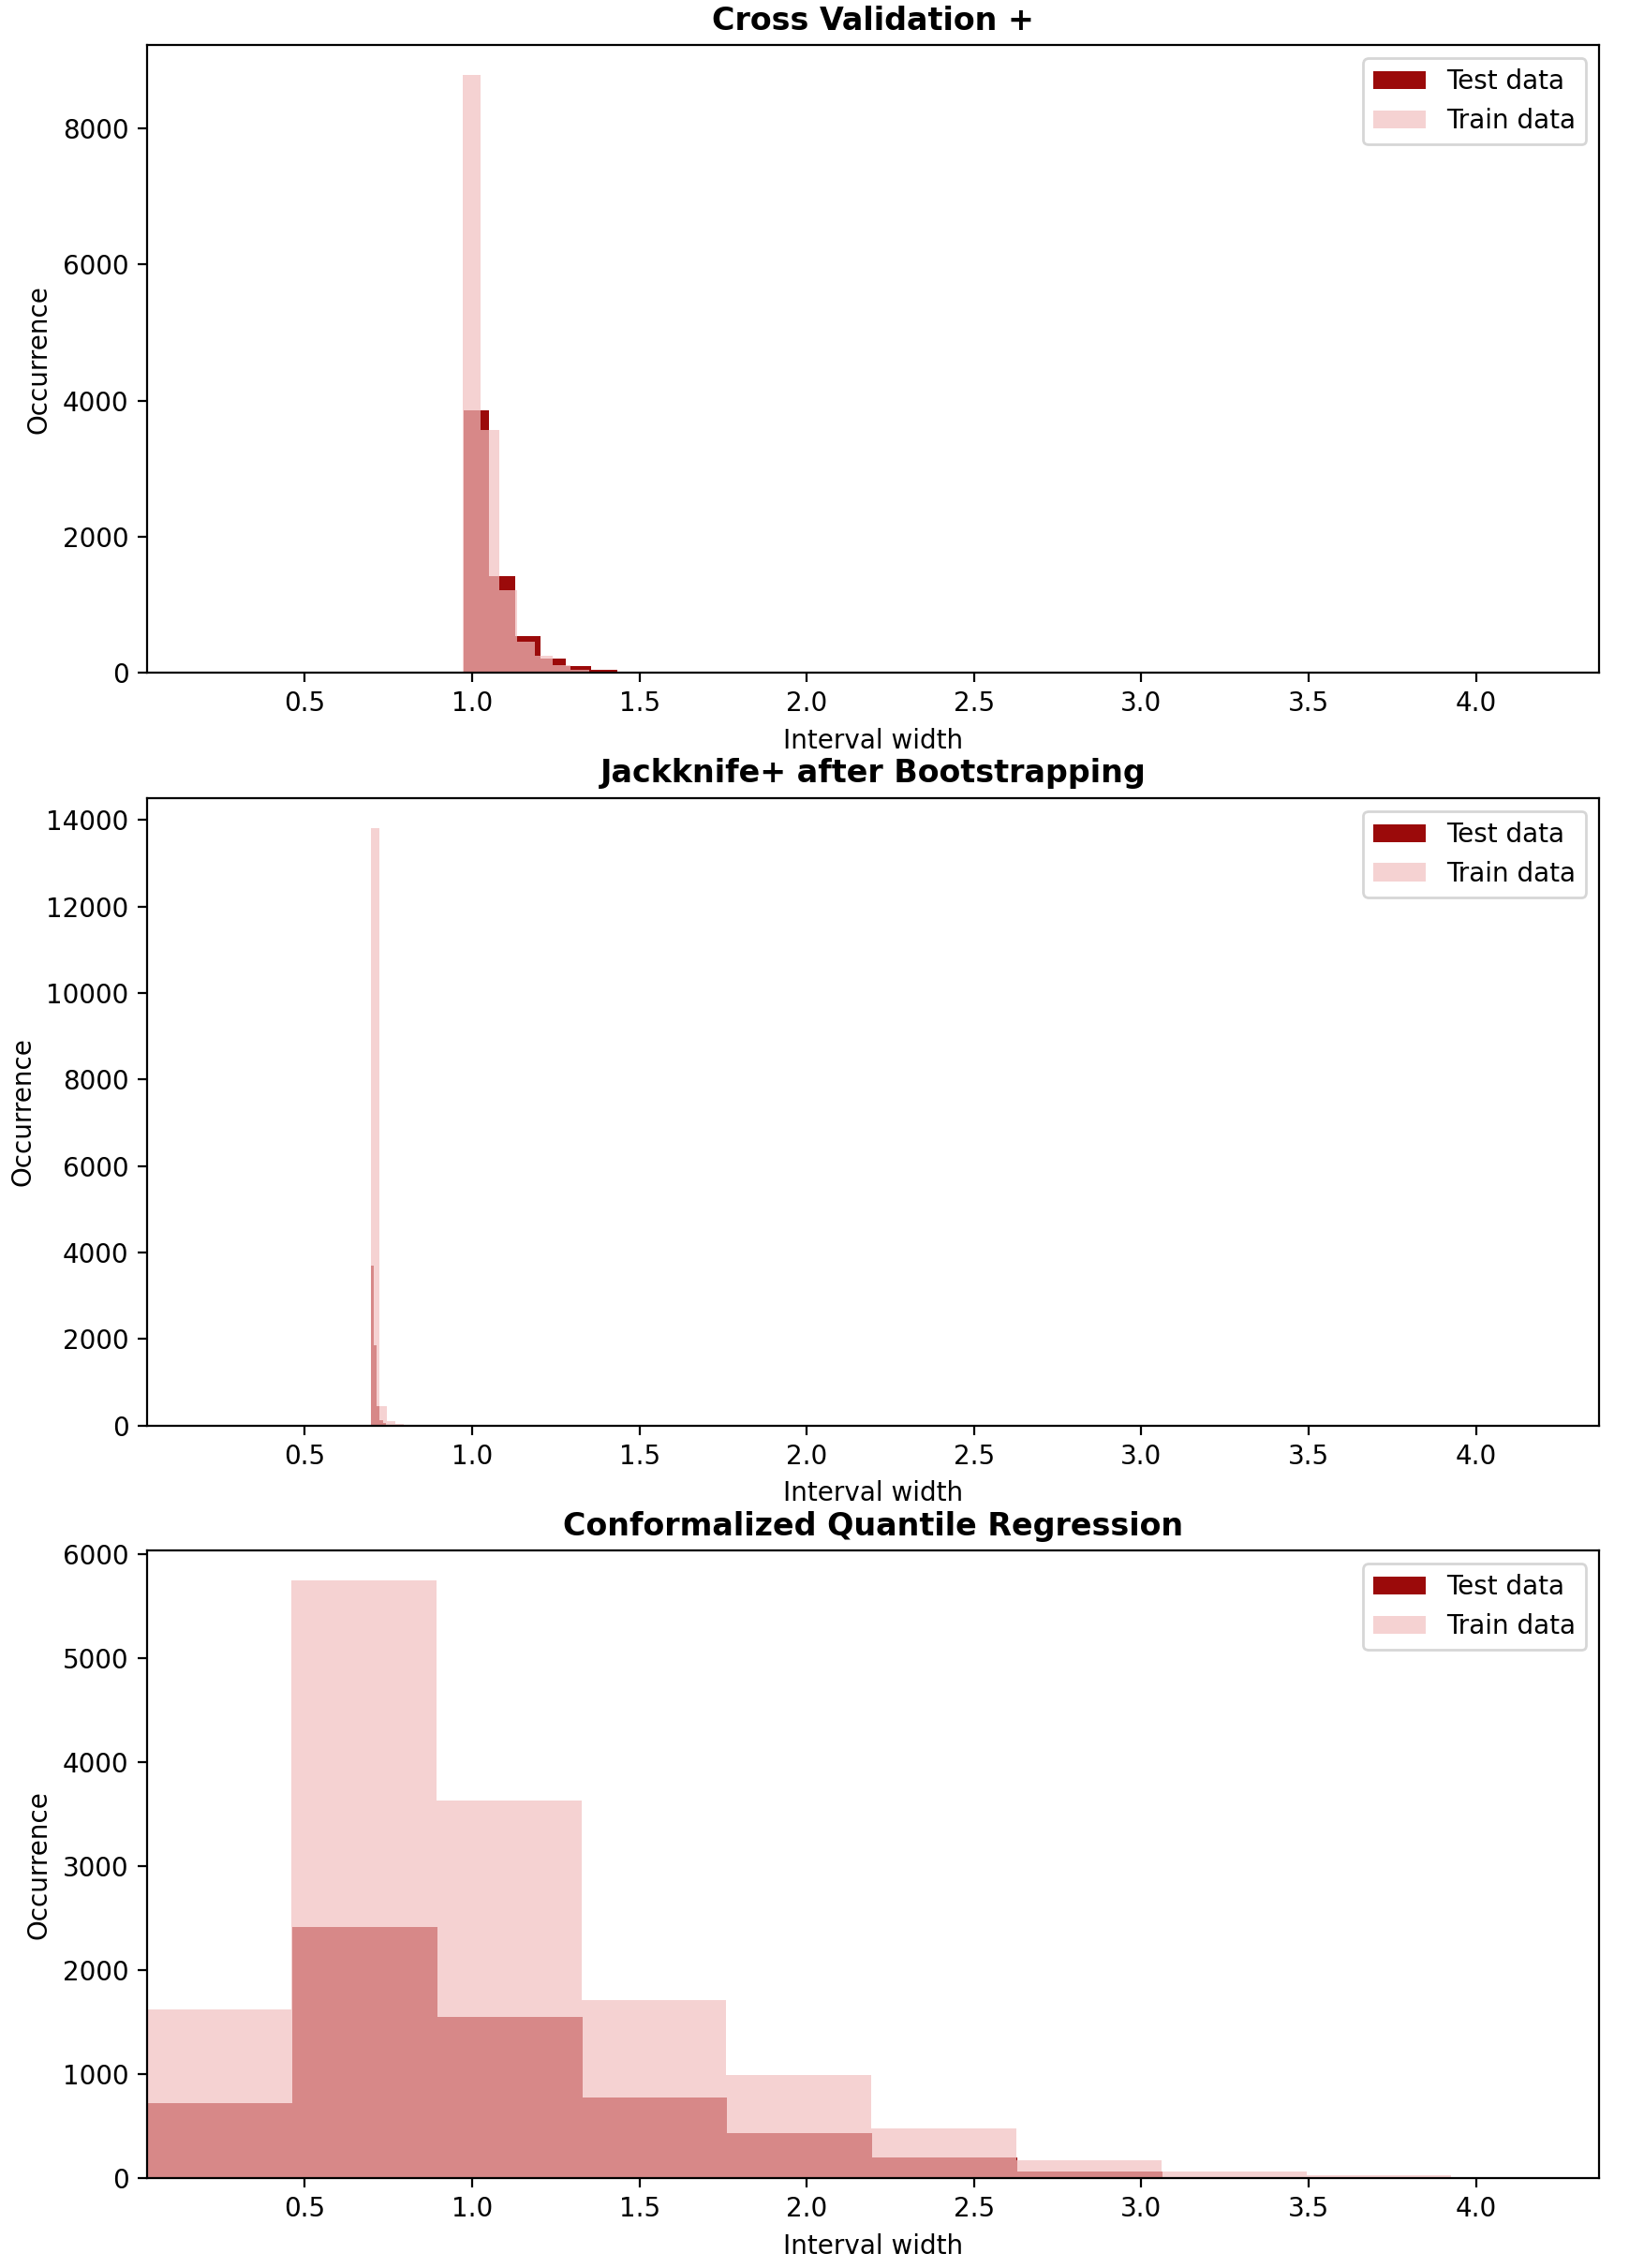
\includegraphics[width=1.15\textwidth, height=2.15\textwidth]{Figures/regression/width-occurrence-regression-problem.png}
        \caption{Intervals' width histograms}
        \label{subfig:regression-width-histograms}
    \end{subfigure}
    \hfill
    \begin{subfigure}[b]{0.32\textwidth}
        \centering
        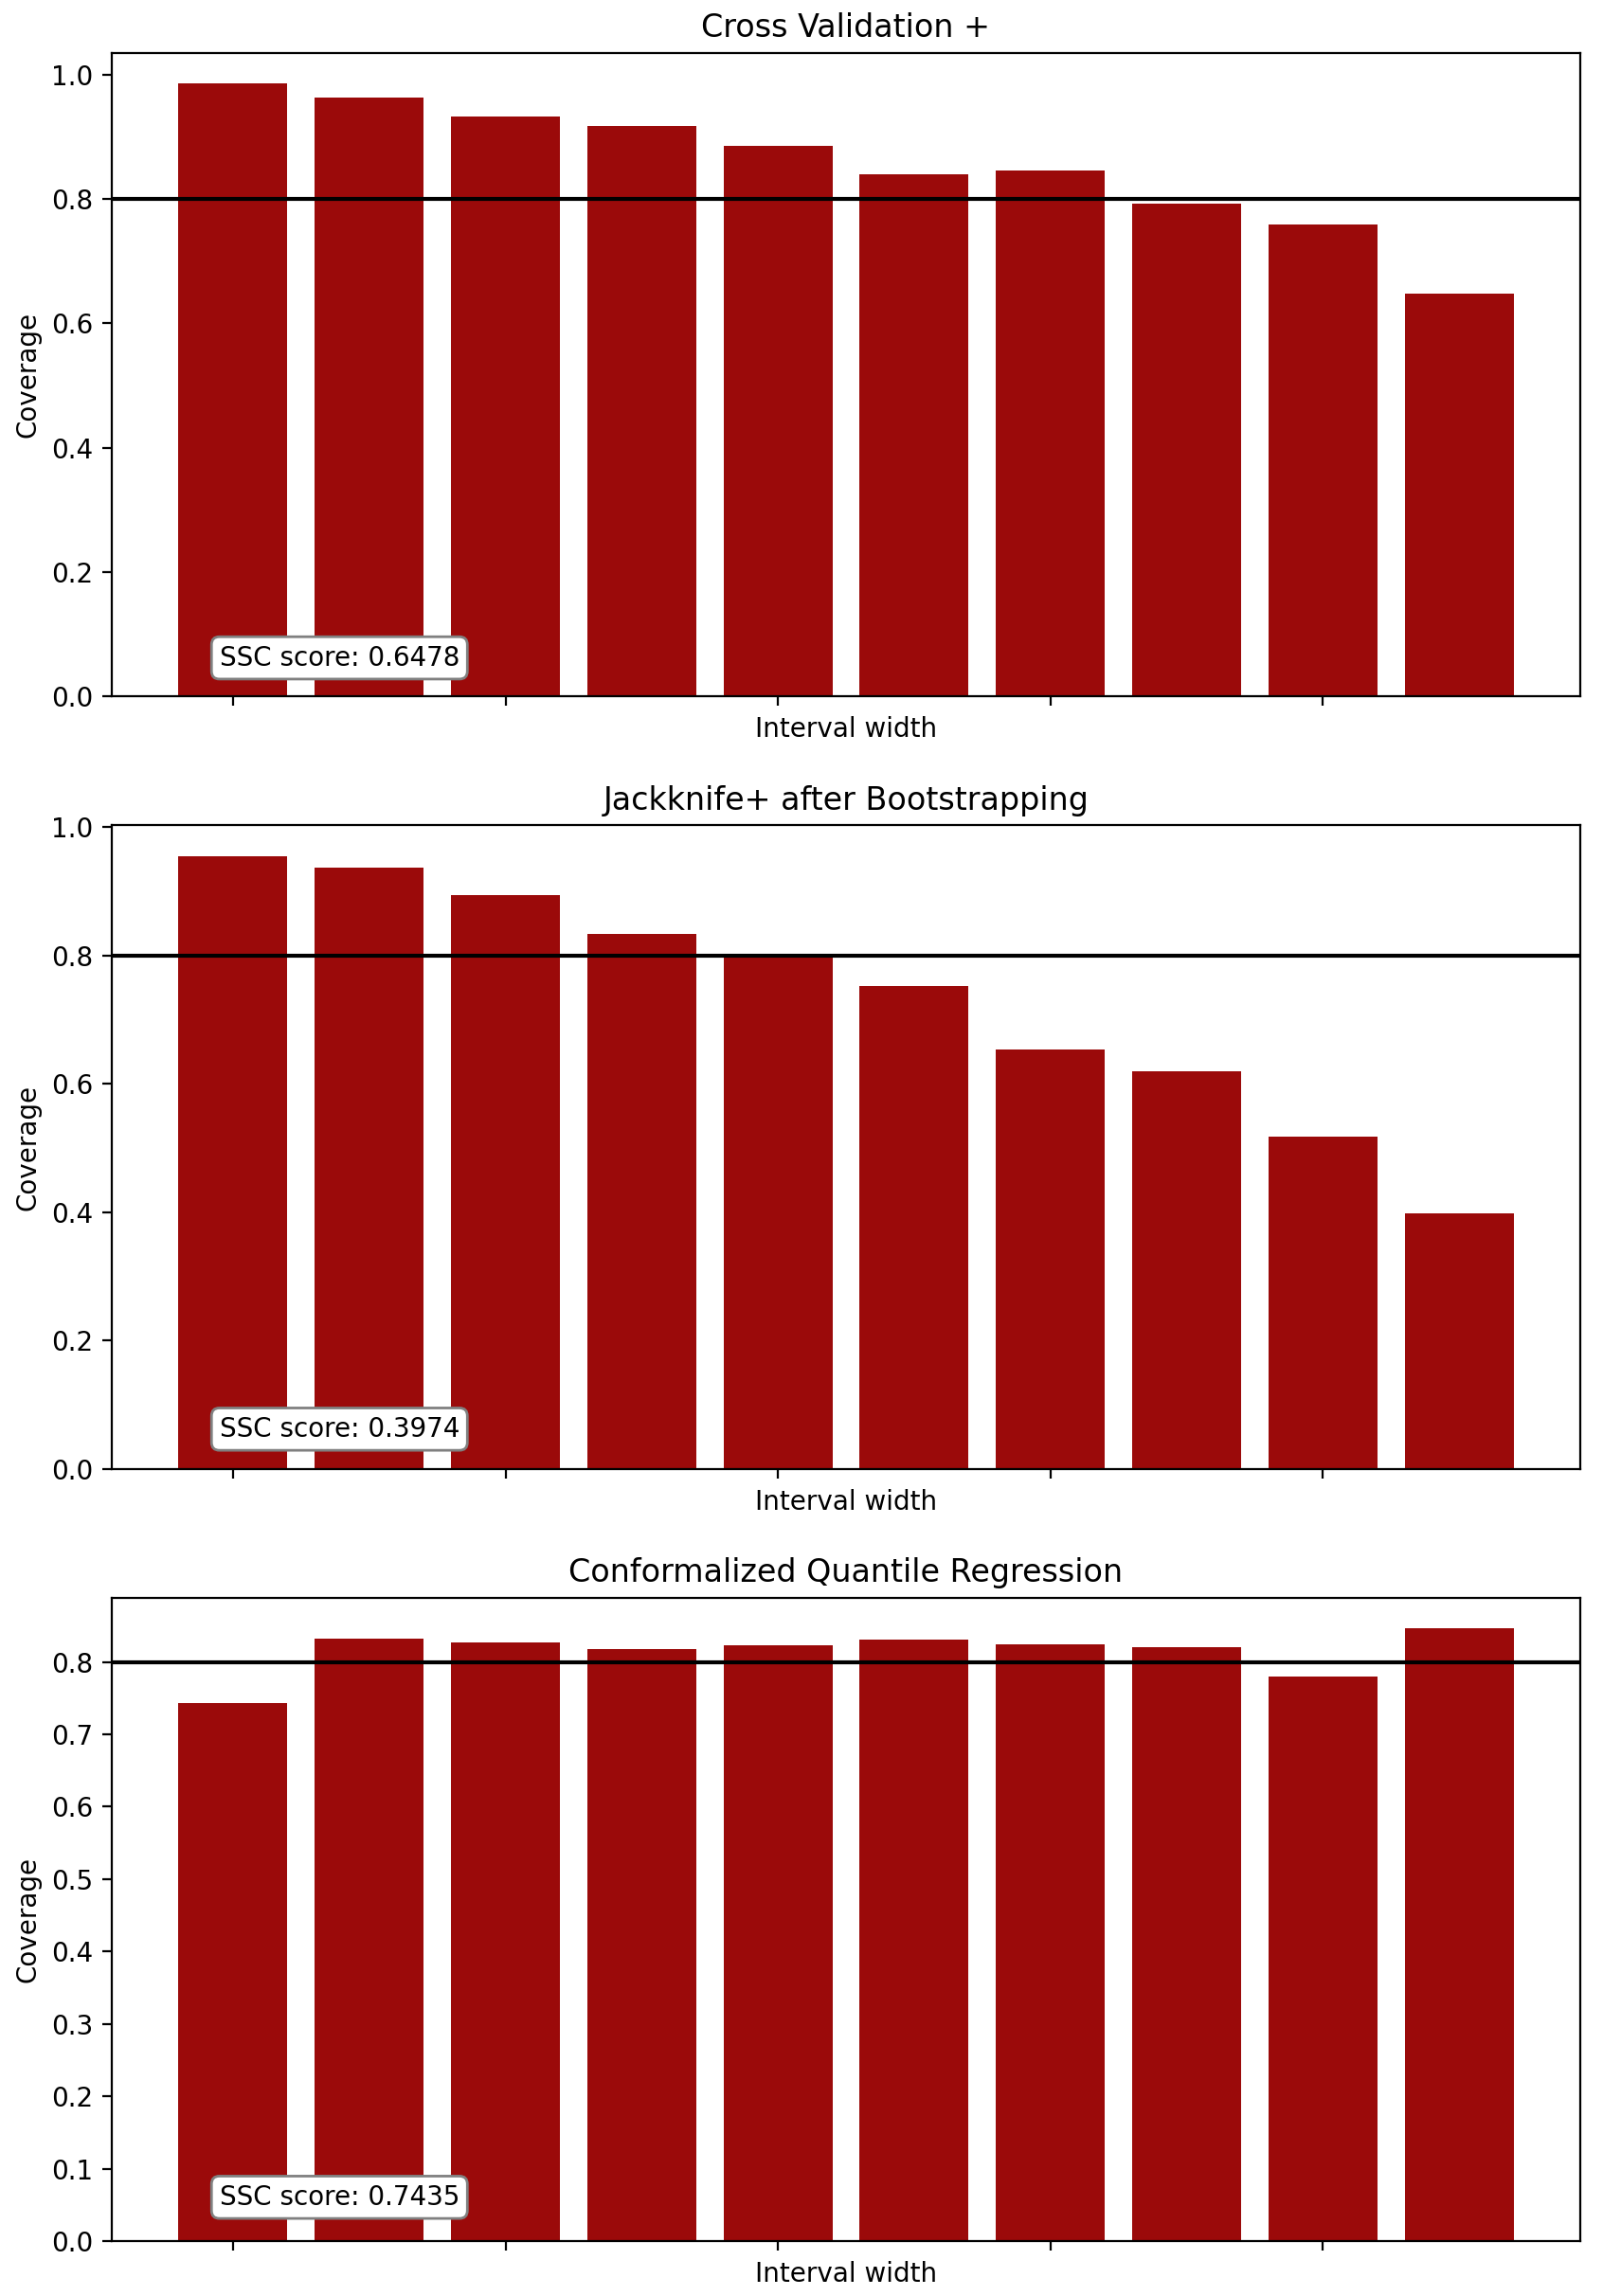
\includegraphics[width=1.15\textwidth, height=2.05\textwidth]{Figures/regression/coverage-vs-width-regression-problem.png}
        \caption{Coverage in function of intervals' width}
        \label{subfig:regression-coverage-width}
    \end{subfigure}
    \hfill % adds horizontal space between figures
    \begin{subfigure}[b]{0.32\textwidth} % Adjust the width to fit your needs
        \centering
        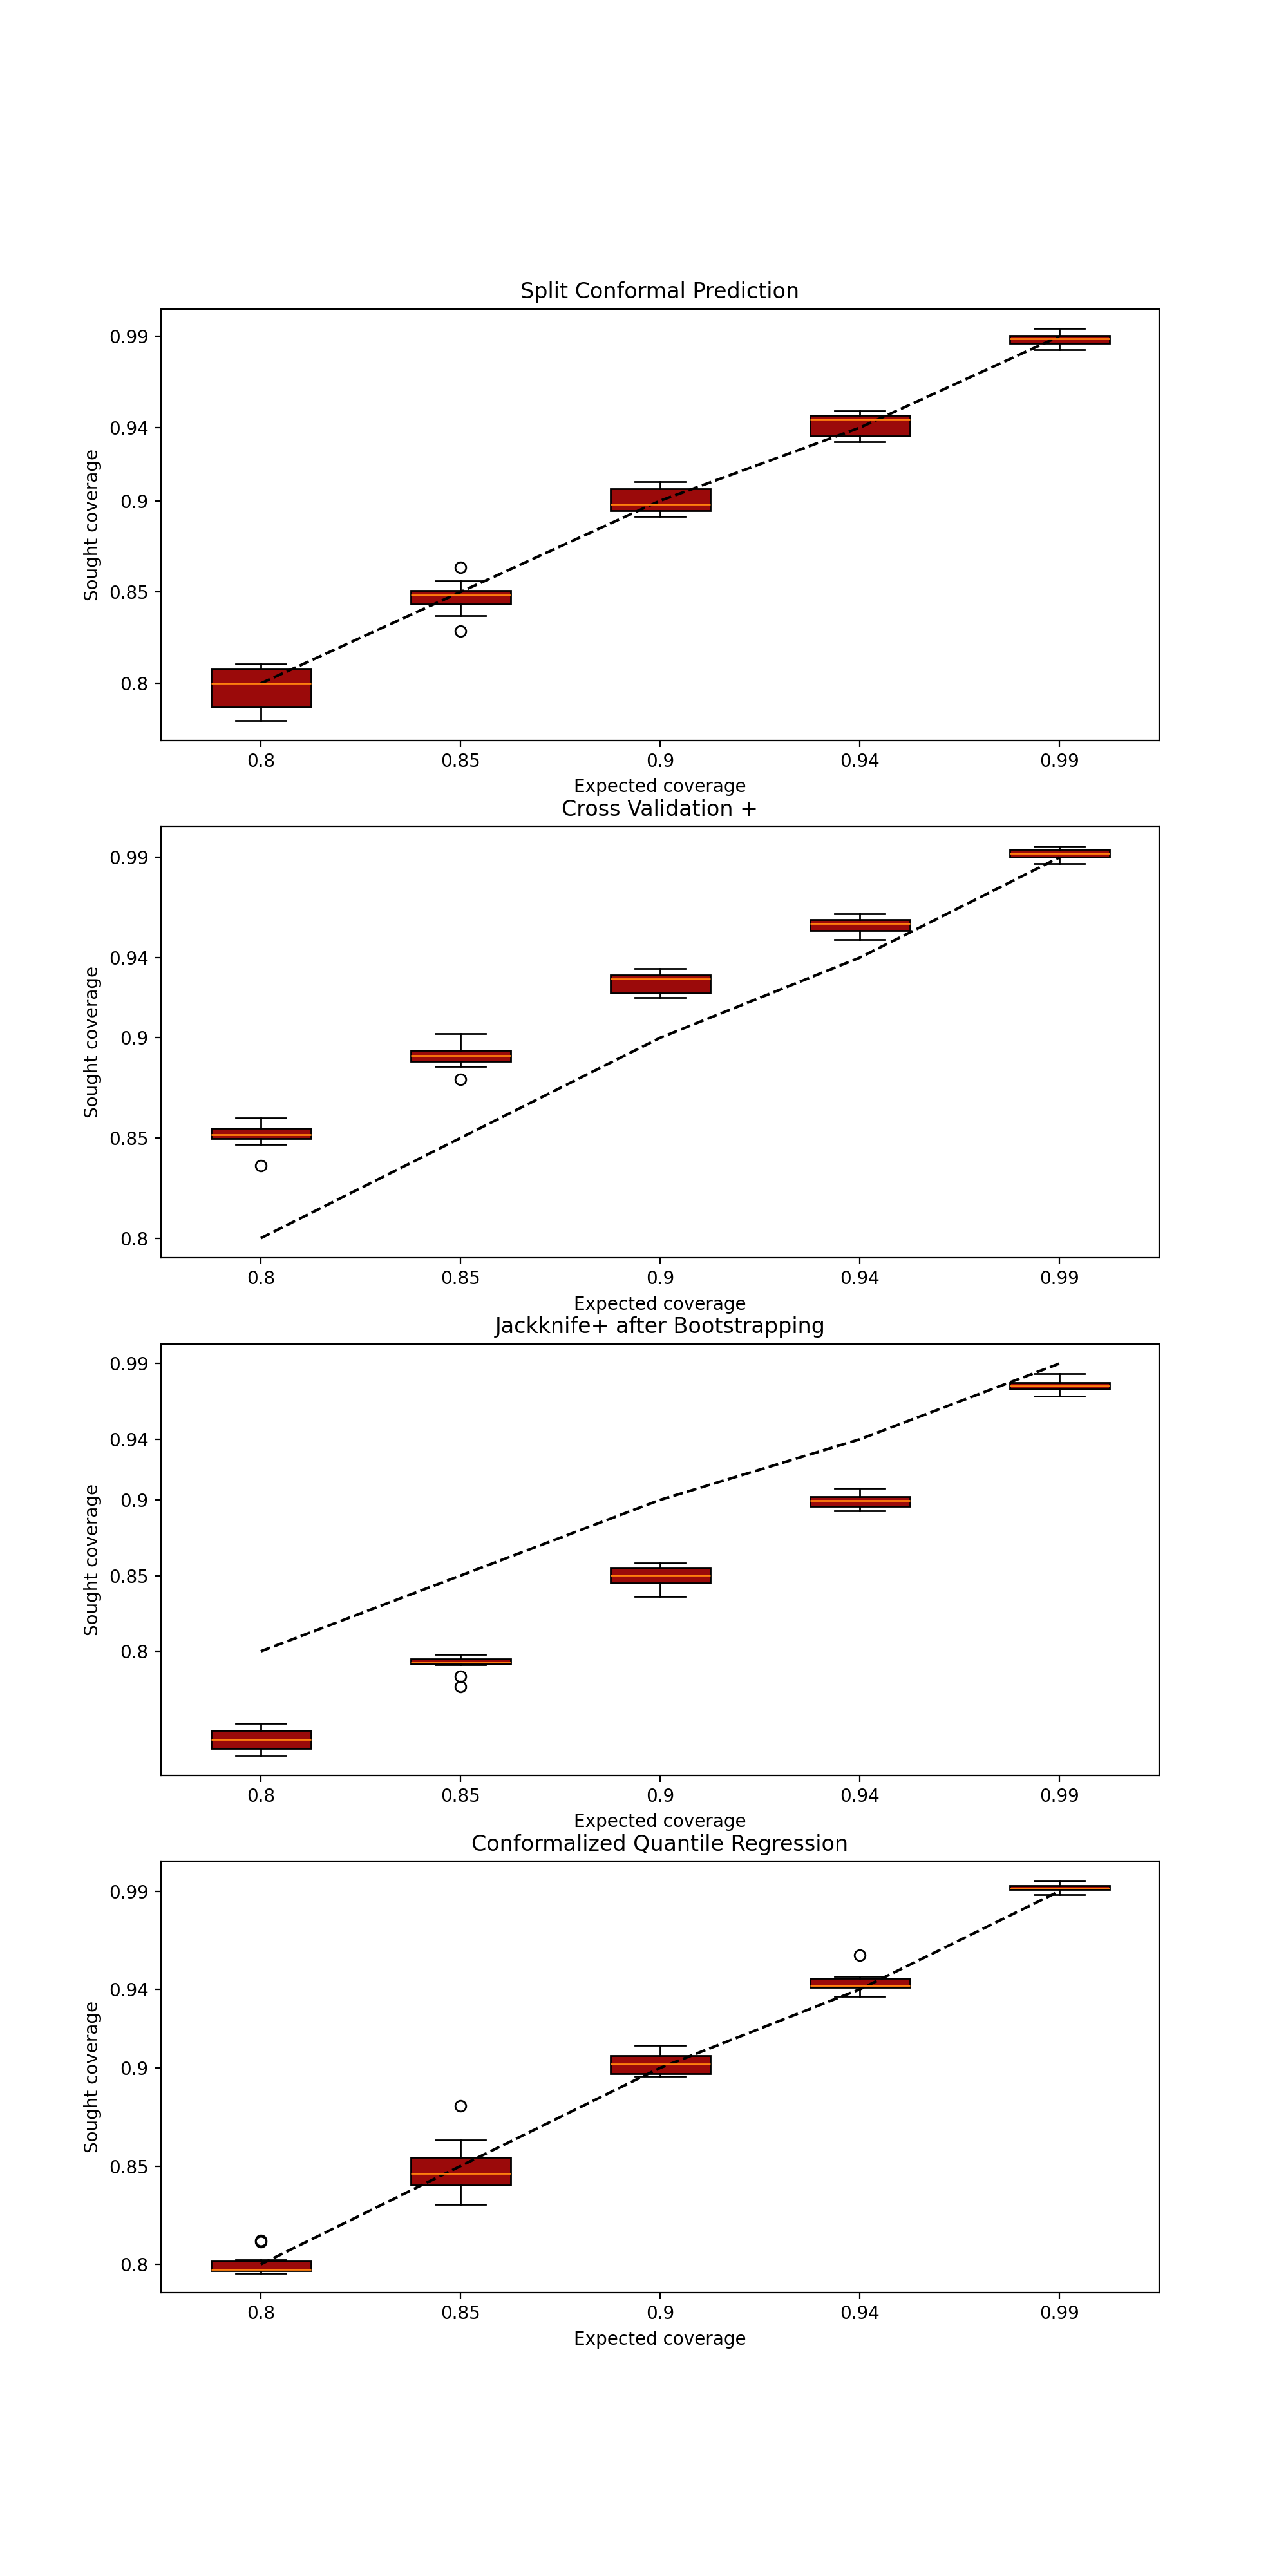
\includegraphics[width=1.15\textwidth, height=3\textwidth]{Figures/regression/coverage-vs-alpha-regression-problem.png} % Adjust the filename and path
        \caption{Coverage in function of $\a$}
        \label{subfig:regression-coverage-alpha}
    \end{subfigure}
    \caption{Visualizations related to width \& coverage distributions for the test data and 4 different strategies, from top to bottom: SCP, CV$+$, J$+$aB \& CQR. The first 2 plots just display the last 3 strategies, since SCP displays no adaptability at all (whereas J$+$aB slight to none adaptability).}
    \label{fig:regression-width-coverage}
\end{figure}

\section{Time series data}\label{sec:results-ts}

For the non-exchangeable data use-case, the same dataset as the \href{https://mapie.readthedocs.io/en/stable/examples_regression/4-tutorials/plot_ts-tutorial.html}{\texttt{mapie}'s time series tutorial} was chosen. This is the Victoria electricity demand dataset, used in the book “\textit{Forecasting: Principles and Practice}” (\cite{hyndman}), and contains a total of 1340 hourly samples. It deals with an electricity demand forecasting problem, which not only features daily and weekly seasonality, but it is also impacted by temperature. Thus, apart from the demand lagged up to 7 days (and other time features), temperature will be used as exogenous variable.

The dataset can be visualized in Figure \ref{fig:app-timeseries-data} at Appendix \ref{app:timeseries-original-problem}, where the complete set of visualizations and plots for the results' analysis can also be found.\\

In this case, a different ensemble model than gradient boosting (section \ref{sec:results-exchangeable}) is chosen as base estimator; in particular, a random forest regressor is implemented through \texttt{sklearn} library's \href{https://scikit-learn.org/stable/modules/generated/sklearn.ensemble.RandomForestRegressor.html}{\texttt{sklearn.ensemble.RandomForestRegressor}} Python class. 

Similarly to section \ref{sec:results-exchangeable}, a randomized grid-search is implemented using a 5-fold cross-validation to automate the hyper-parameters fine-tuning task. For this particular problem, the found best settings are:
\begin{itemize}
    \setlength{\itemsep}{0pt}
    \item \texttt{max\_{}depth}: $23$
    \item \texttt{n\_{}estimators}: $99$
\end{itemize}

Then, 2 strategies based in \texttt{mapie}'s \texttt{EnbPI} implementation (see the configuration at section \ref{sec:implementation}) are implemented, these are: \texttt{EnbPI} without partial fit (EnbPI\_{}nP), \textit{i.e.} the test residuals are not used to further adjust the model (steps 15-19 of Algorithm \ref{alg:EnbPI}); and \texttt{EnbPI} with partial fit (EnbPI).

In both cases, the prediction batches were implemented using the \texttt{mapie}'s class for bootstrapping blocks of data, \href{https://mapie.readthedocs.io/en/latest/generated/mapie.subsample.BlockBootstrap.html}{\texttt{mapie.subsample.BlockBootstrap}}, with:
\begin{itemize}
    \setlength{\itemsep}{0pt}
    \item \texttt{n\_{}resamplings}$=100$
    \item \texttt{length}$=48$ (i.e. batch size of $s=48\ \mathrm{h}$ samples).
\end{itemize}

All the code used to generate these results and visualizations can be found at the author's \href{https://github.com/gcastro-98/conformal-prediction/blob/main/timeseries.ipynb}{timeseries.ipynb} notebook.

\subsection{Original dataset}\label{subsec:timeseries-original}

For the original Victoria electricity demand dataset, both EnbPI\_{}nP and EnbPI are able to provide informative prediction intervals, presenting some minor differences in their attributes as shown in Table \ref{tab:timeseries-metrics}.

\begin{table}[ht]
\centering

\begin{subtable}{.5\textwidth}
    \hspace{-28mm}
    \begin{tabular}{|c|c|c|c|}
    \rowcolor{ColHead}\textcolor{white}{Strategy} & \textcolor{white}{Coverage} & \textcolor{white}{RMSE} & \textcolor{white}{Total time  (train $+$ infer)} \\ \hline
    \cellcolor{RowHead}EnbPI\_{}nP & 0.780 $\pm$ 0.069 & 0.165 $\pm$ 0.067 & 6.157 $\pm$ 0.334 \\
    \cellcolor{RowHead}EnbPI & 0.789 $\pm$ 0.058 & 0.165 $\pm$ 0.067 & 528.343 $\pm$ 0.359\\
    \hline
    \end{tabular}
\caption{Coverage, RMSE, total time (training \& inference with residuals adjustment if applies).}
\label{subtab:timeseries-metrics-1}
\end{subtable}

\begin{subtable}{.5\textwidth}
    \hspace{-28mm}
    \begin{tabular}{|c|c|c|c|c|}
    \rowcolor{ColHead}\textcolor{white}{Strategy} & \textcolor{white}{Coverage} & \textcolor{white}{Width} & \textcolor{white}{CWC} & \textcolor{white}{SSC} \\ \hline
    \cellcolor{RowHead}EnbPI\_{}nP & 0.780 $\pm$ 0.069 & 0.293 $\pm$ 0.013 & 0.935 $\pm$ 0.018 & ---  \\
    \cellcolor{RowHead}EnbPI & 0.789 $\pm$ 0.058 & 0.300 $\pm$ 0.007 & 0.934 $\pm$ 0.016 & 0.518 $\pm$ 0.209\\
    \hline
    \end{tabular}
\caption{Coverage, width, coverage width-based criterion (CWC) score \& size-stratified coverage (SSC) score}
\label{subtab:timeseries-metrics-2}
\end{subtable}

\caption{Different strategies' metrics after the Figure \ref{fig:ts-5-folds}'s 5-fold cross-validation for the time series problem with $\a=0.2$.}
\label{tab:timeseries-metrics}
\end{table}

Note these results stem from a 5-fold cross-validation, with the batches (not shuffled samples, to break temporal auto-correlation) shown in Figure \ref{fig:ts-5-folds}.

\begin{figure}[ht]
    %\centering
    \hspace{-10mm}
    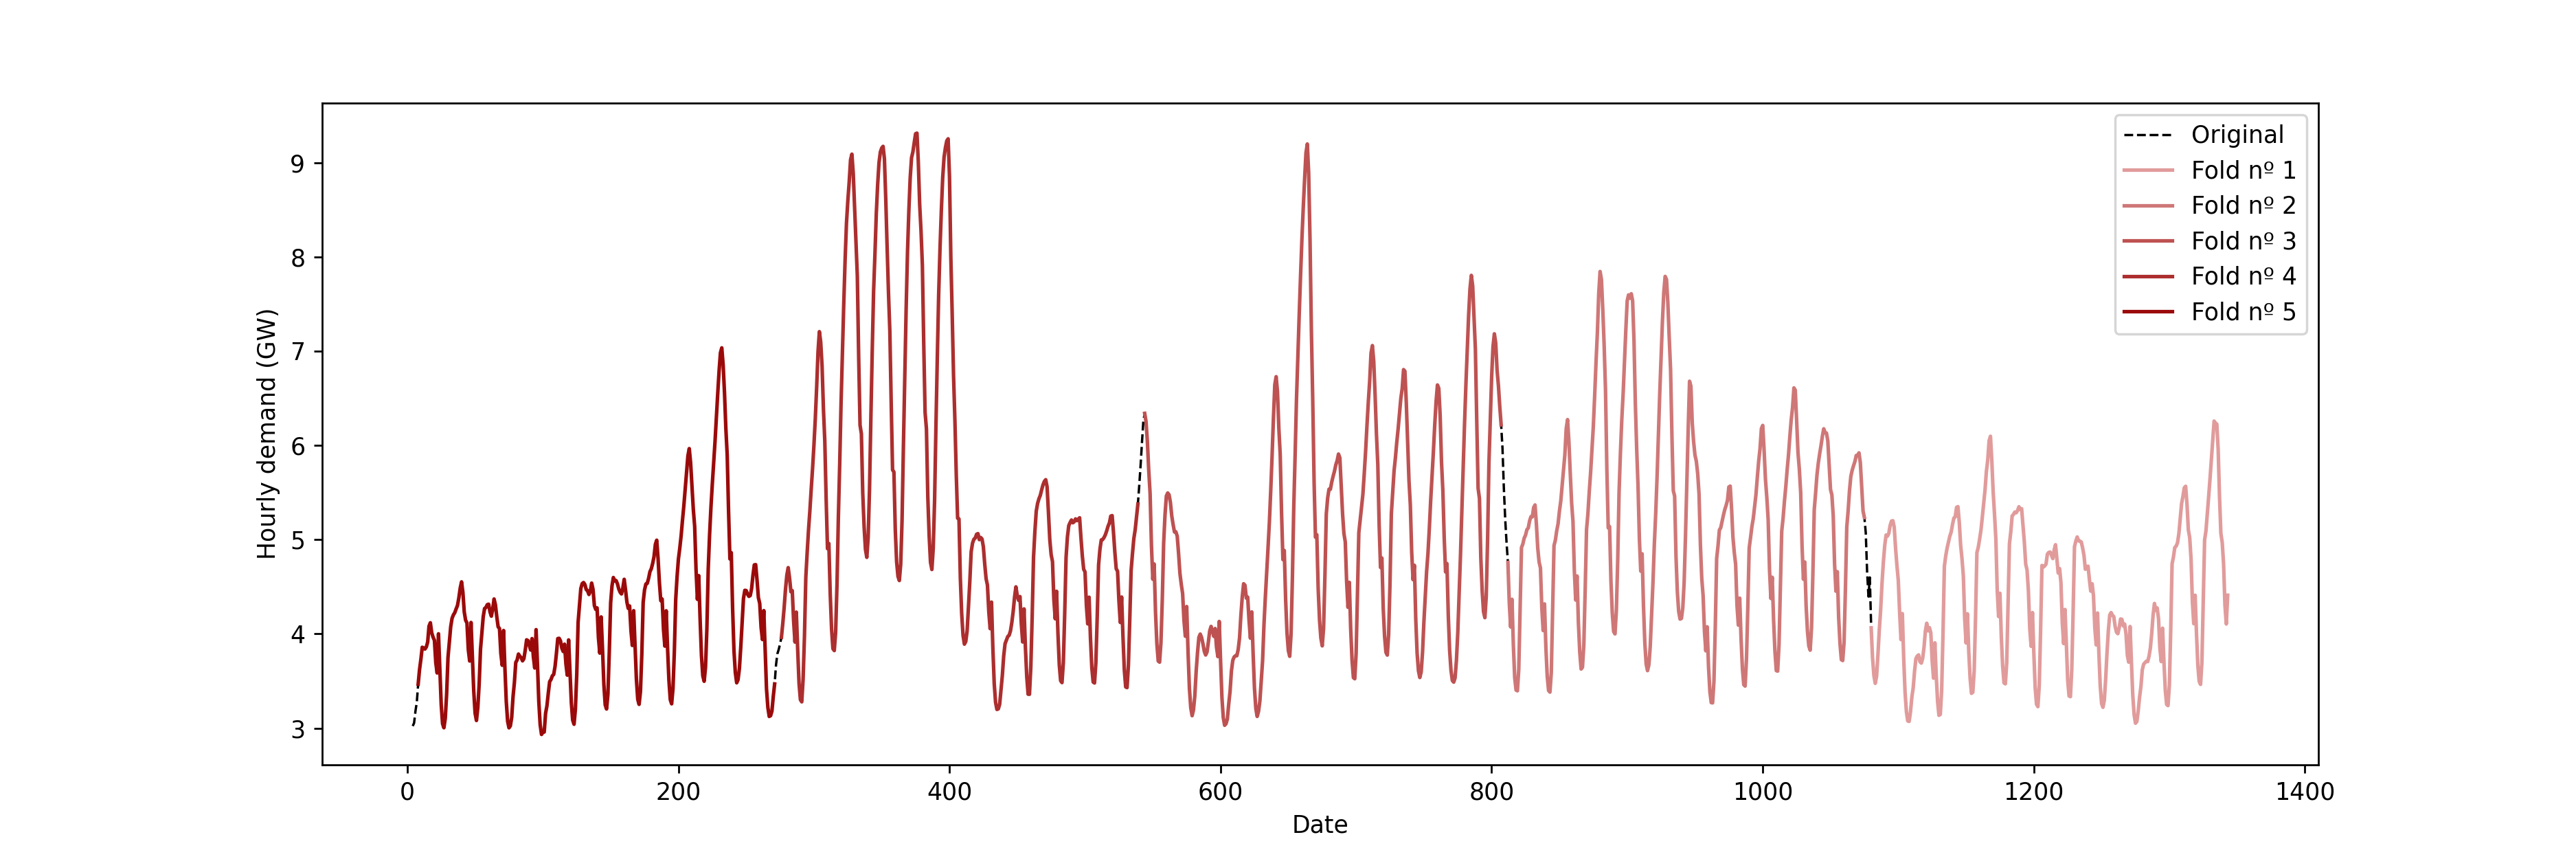
\includegraphics[width=1.15\textwidth]{Figures/timeseries/without-change-point/ts-5-folds.png}
    \caption{5-fold splits from the original dataset.}
    \label{fig:ts-5-folds}
\end{figure}

In particular, it is easy to conclude the benefits of adjusting the intervals with the test residuals (steps 15-19 of Algorithm \ref{alg:EnbPI}) since EnbPI is better than EnbPI\_{}nP. Despite a slight $0.001$ loss width-coverage ratio score, the global coverage improved. Not only global coverage was improved, but also adaptive intervals were enabled achieving a $0.518\pm 0.209$ SSC score (with respect to the non-adaptive intervals of EnbPI\_{}nP).

The latter can be easily checked in sub-figures \ref{subfig:timeseries-width-histograms} \& \ref{subfig:timeseries-coverage-width}, where not only EnbPI features several sized intervals, but it also attains uniform coverage in every of them (and almost the expected one). Also, the ability to attain global coverage for different $\a$ values is shown in sub-figure \ref{subfig:timeseries-coverage-alpha}.

\begin{figure}[ht]
    \centering
    %\hspace{-10mm}
    \begin{subfigure}[b]{0.32\textwidth}
        \centering
        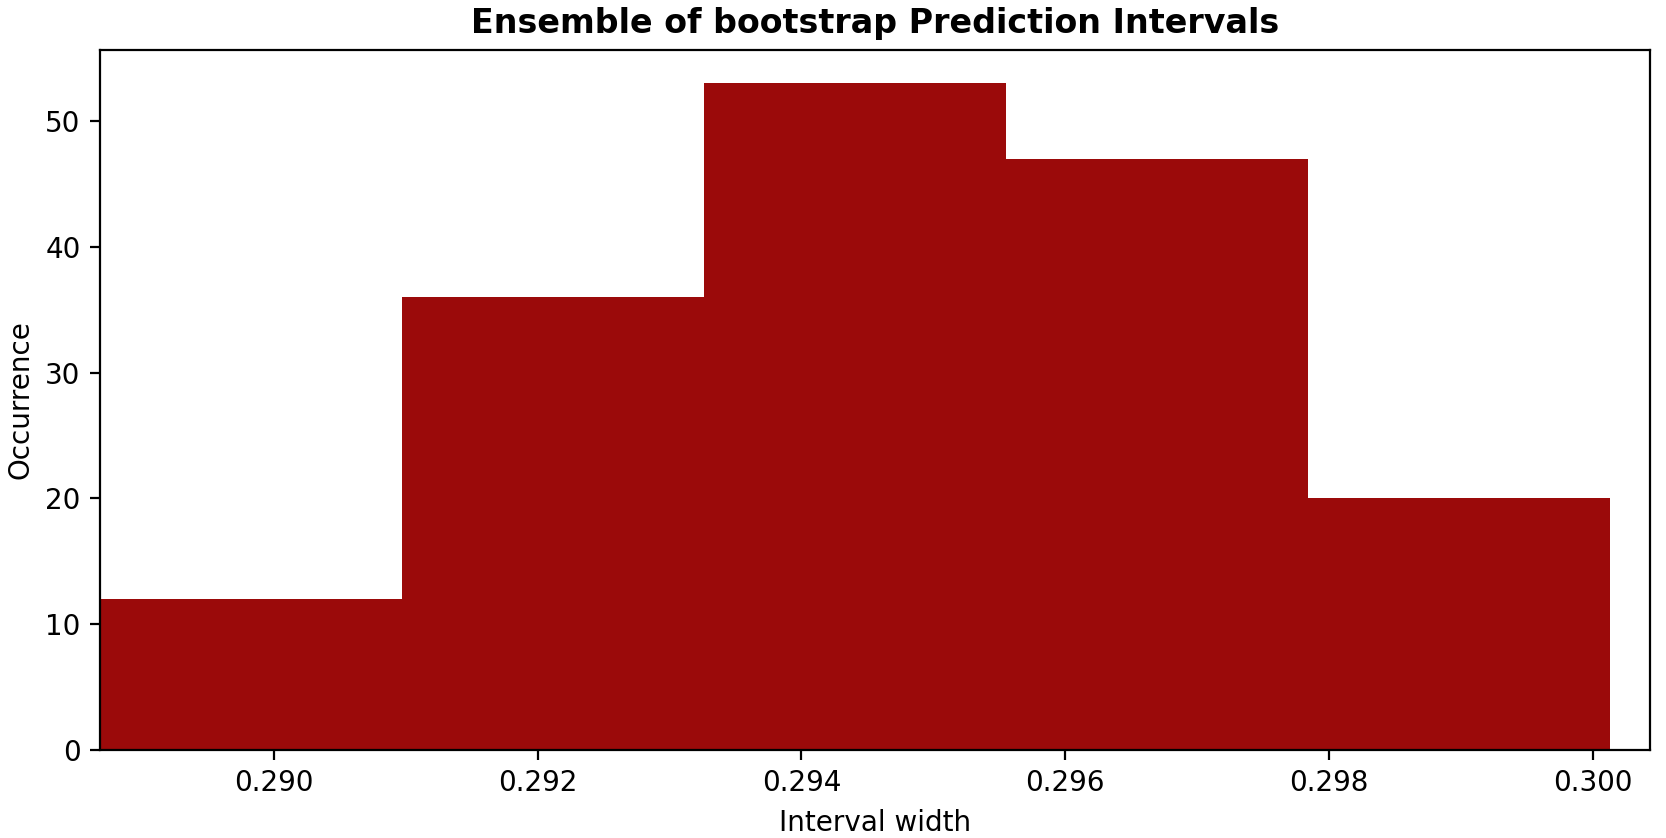
\includegraphics[width=1.05\textwidth, height=0.85\textwidth]{Figures/timeseries/without-change-point/width-occurrence-timeseries-problem.png}
        \caption{Intervals' width histograms}
        \label{subfig:timeseries-width-histograms}
    \end{subfigure}
    \hfill
    \begin{subfigure}[b]{0.32\textwidth}
        \centering
        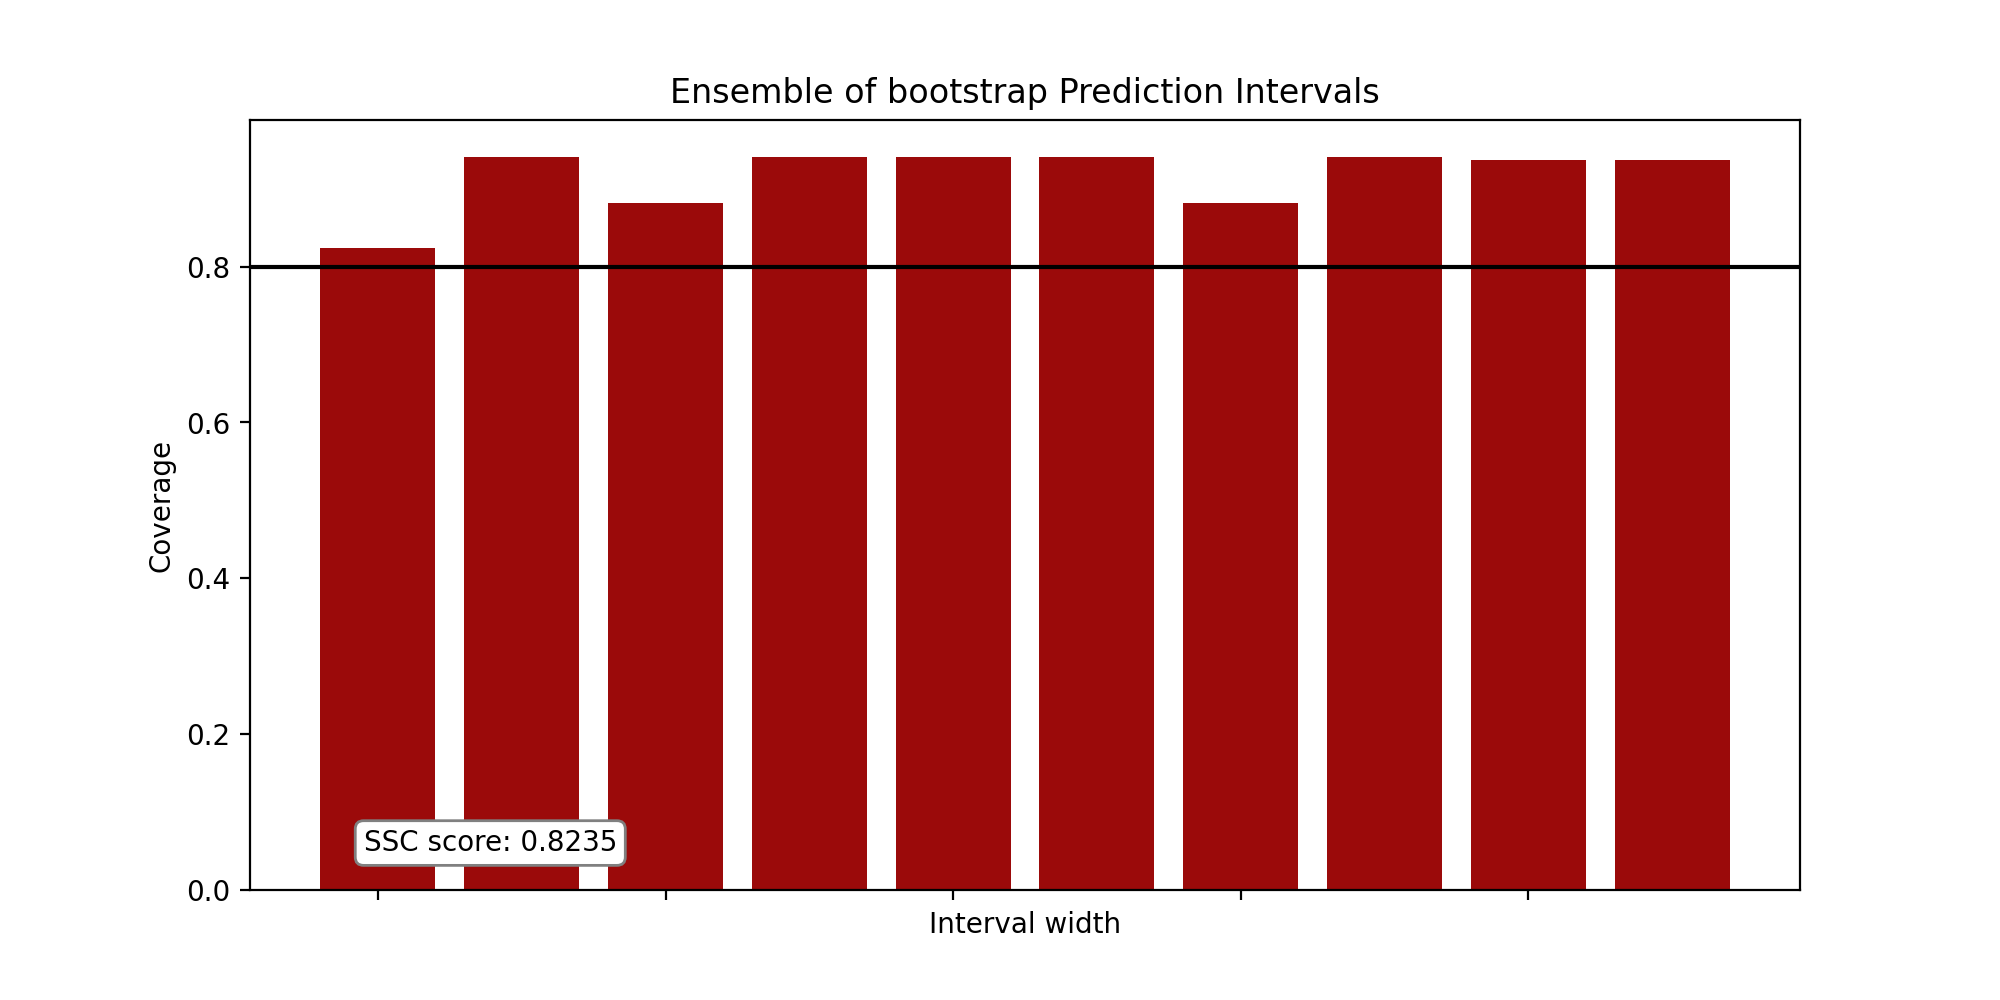
\includegraphics[width=1.15\textwidth, height=0.85\textwidth]{Figures/timeseries/without-change-point/coverage-vs-width-timeseries-problem.png}
        \caption{Coverage in function of intervals' width}
        \label{subfig:timeseries-coverage-width}
    \end{subfigure}
    \hfill % adds horizontal space between figures
    \begin{subfigure}[b]{0.32\textwidth} % Adjust the width to fit your needs
        \centering
        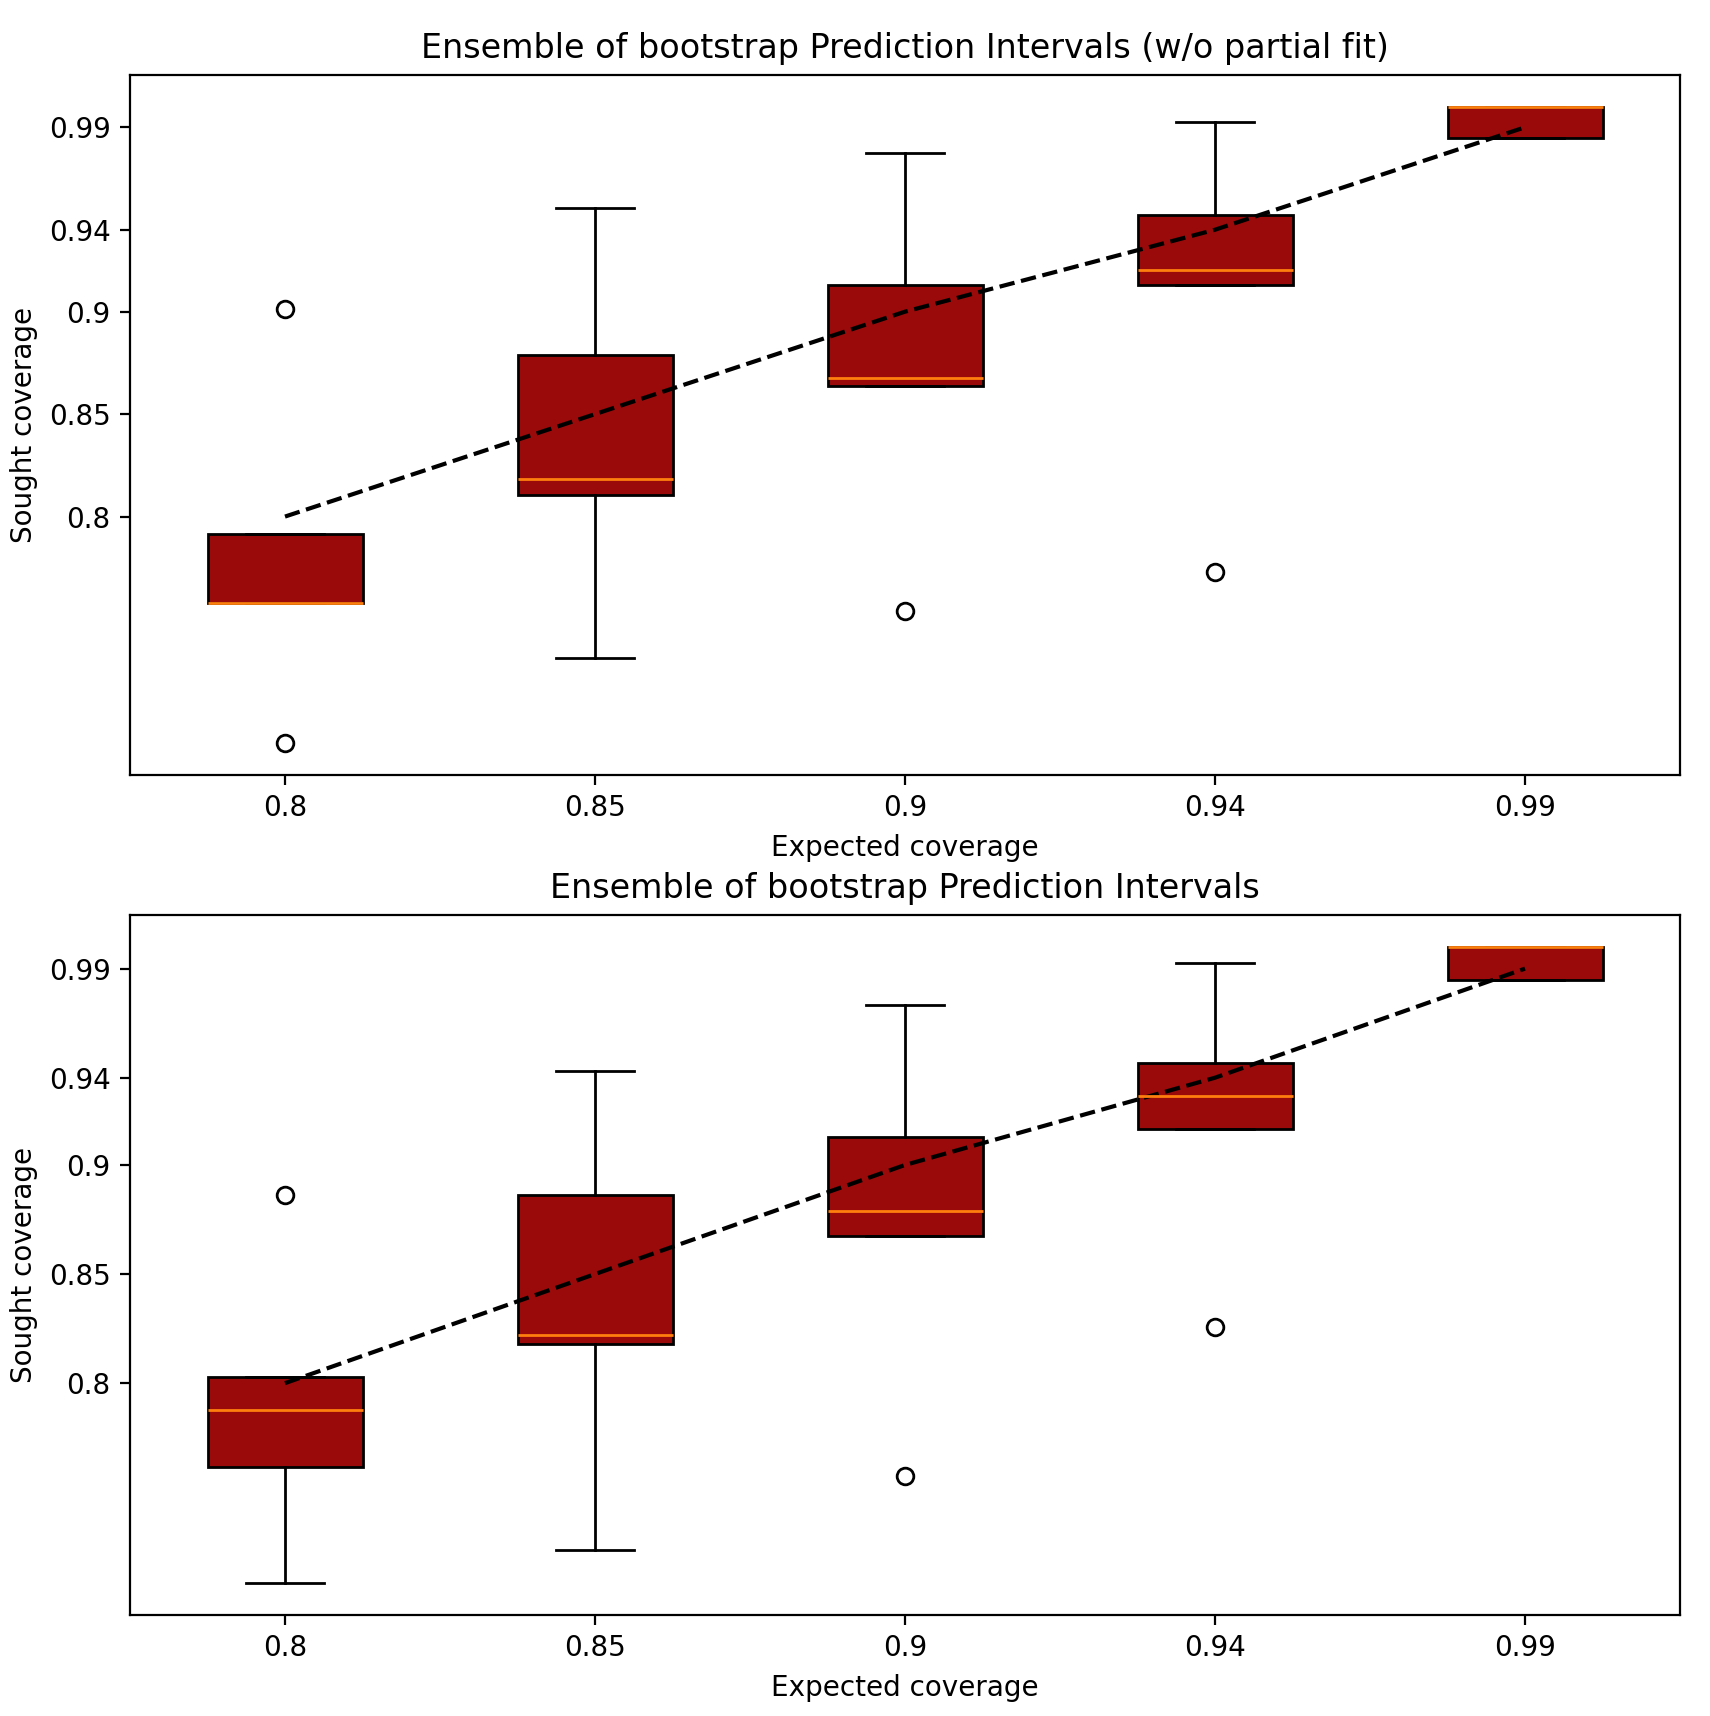
\includegraphics[width=1.15\textwidth, height=1.75\textwidth]{Figures/timeseries/without-change-point/coverage-vs-alpha-timeseries-problem.png} % Adjust the filename and path
        \caption{Coverage in function of $\a$}
        \label{subfig:timeseries-coverage-alpha}
    \end{subfigure}
    \caption{Intervals width \& coverage distributions for the test data and the EnbPI strategy (without partial fit, top; and with it, bottom).}
    \label{fig:timeseries-width-coverage}
\end{figure}

Of course, despite its complexity and multiple seasonality, this dataset is very consistent presenting almost neither trend nor strong distribution shifts as shown in Figure \ref{fig:ts-5-folds}. Due to this reason, EnbPI\_{}nP \& EnbPI performances are really similar.

To avoid outshining EnbPI adaptive ability, a special strong-shift case is presented in subsection \ref{subsec:ts-with-cpoint}.

\subsection{Change point in the test data}\label{subsec:ts-with-cpoint}

Henceforth in this subsection, a special case of the time series problem is considered. In particular, a change point will be added in the test split (by artificially subtracting $2\ \mathrm{GW}$) to mock off the situation in which there is a sudden strong distribution shift in the middle of the test data. Also, in this case and unless otherwise is specified, $\a=0.05$ is chosen as miscoverage level.

The dataset with this change point can be visualized in Figure \ref{fig:app-timeseries-data-cpoint} at Appendix \ref{app:timeseries-cpoint-problem} (where the rest of visualizations can also be found).\\

For this particular scenario, EnbPI\_{}nP and EnbPI do present significance differences in their performance, as shown in Table \ref{tab:timeseries-metrics-cpoint}.

\begin{table}[ht]
\centering

\begin{subtable}{.5\textwidth}
    \hspace{-28mm}
    \begin{tabular}{|c|c|c|c|}
    \rowcolor{ColHead}\textcolor{white}{Strategy} & \textcolor{white}{Coverage} & \textcolor{white}{RMSE} & \textcolor{white}{Total time (train $+$ infer)} \\ \hline
    \cellcolor{RowHead}EnbPI\_{}nP & 0.439 $\pm$ 0.075 & 1.431 $\pm$ 0.024 & 6.047 $\pm$ 0.307 \\
    \cellcolor{RowHead}EnbPI & 0.696 $\pm$ 0.042 & 1.431 $\pm$ 0.024 & 529.902 $\pm$ 1.319\\
    \hline
    \end{tabular}
\caption{Coverage, RMSE, total time (training \& inference with residuals adjustment if applies).}
\label{subtab:timeseries-metrics-1-cpoint}
\end{subtable}

\begin{subtable}{.5\textwidth}
    \hspace{-18mm}
    \begin{tabular}{|c|c|c|c|}
    \rowcolor{ColHead}\textcolor{white}{Strategy} & \textcolor{white}{Coverage} & \textcolor{white}{Width} %& \textcolor{white}{CWC} 
    & \textcolor{white}{SSC} \\ \hline
    \cellcolor{RowHead}EnbPI\_{}nP & 0.439 $\pm$ 0.075 & 0.569 $\pm$ 0.043 % & --- %0.899 $\pm$ 0.031 
    & ---  \\
    \cellcolor{RowHead}EnbPI & 0.696 $\pm$ 0.042 & 1.300 $\pm$ 0.034 % & --- %0.777 $\pm$ 0.060 
    & 0.069 $\pm$ 0.120\\
    \hline
    \end{tabular}
\caption{Coverage, width % , %coverage width-based criterion (CWC) score 
\& size-stratified coverage (SSC) score.}
\label{subtab:timeseries-metrics-2-cpoint}
\end{subtable}

\caption{Different strategies' metrics after the Figure \ref{fig:ts-5-folds-cpoint}'s 5-fold cross-validation for the time series problem (with a change point in test) and $\a=0.05$.}
\label{tab:timeseries-metrics-cpoint}
\end{table}

Note these metrics are obtained from the batched 5-fold cross-validation splits shown in Figure \ref{fig:ts-5-folds-cpoint} (just the test splits are shown, the train split is the rest of the dataset for each case).

\begin{figure}[ht]
    \hspace{-12mm}
    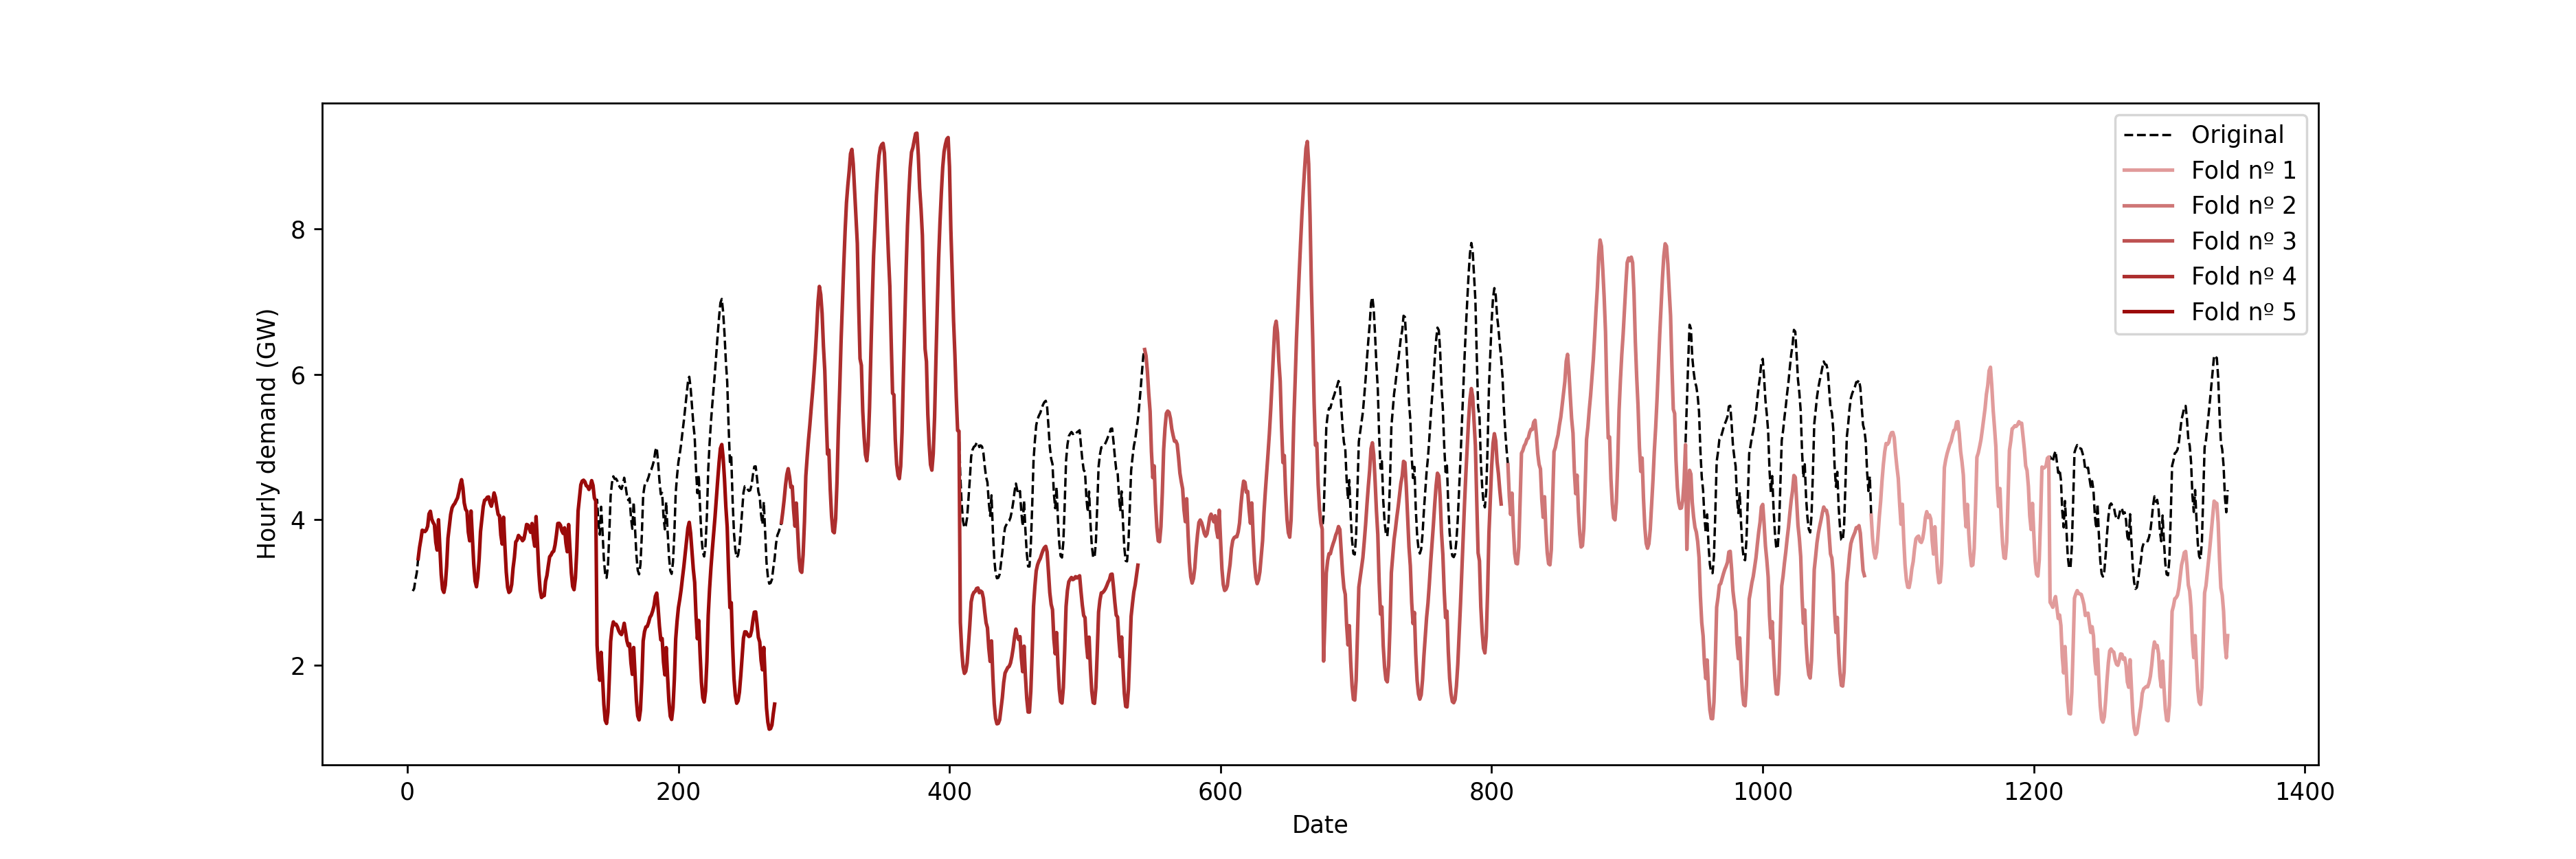
\includegraphics[width=1.15\textwidth]{Figures/timeseries/with-change-point/ts-with-change-point-5-folds.png}
    \caption{5-fold splits from the dataset with change point in the test split(s).}
    \label{fig:ts-5-folds-cpoint}
\end{figure}

These results clearly justify the need of adjusting the intervals with the test residuals (EnbPI) despite of significantly increasing the computational times.\\

Specifically, EnbPI's ability of increasing the intervals width after the strong-shift in the middle of the test split, allows the methodology to recover and yields a $58.54\%$ coverage increase. This justified need of suddenly increasing intervals width (making them less informative) is the reason why the CWC score is not shown in Table \ref{tab:timeseries-metrics-cpoint}, since it could lead to wrong interpretations (the metric would penalize this behavior).

This behavior by which EnbPI, and after the change point, tries to compensate the lack of coverage in their future predictions (by increasing intervals width) is easily observed at Figure \ref{fig:timeseries-prediction-intervals-cpoint}.\\

\begin{figure}[ht]
    \centering
    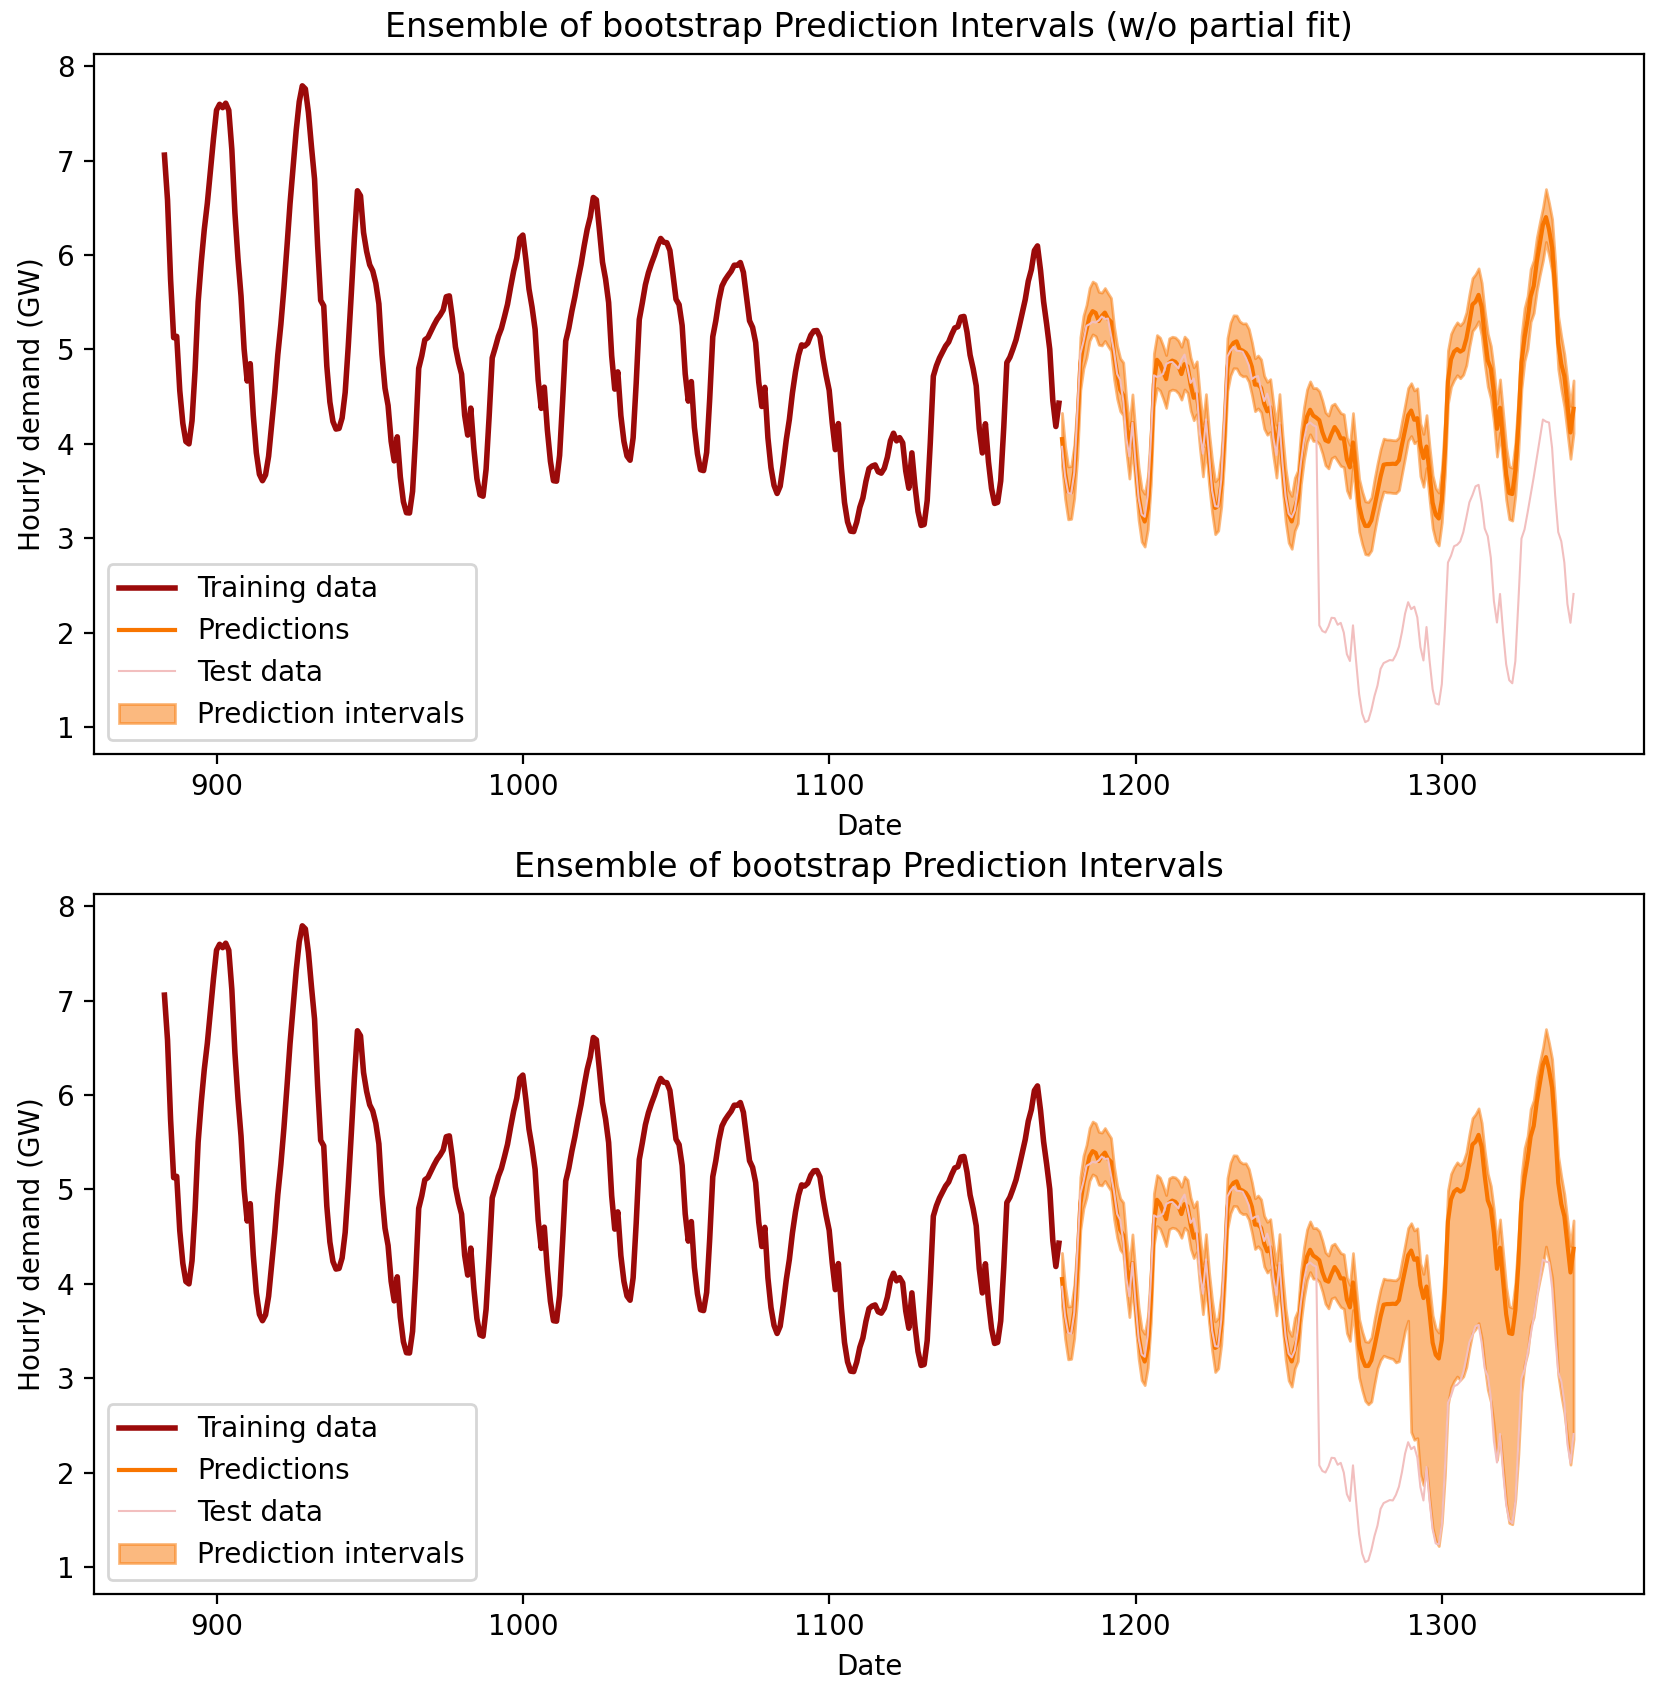
\includegraphics[width=\textwidth]{Figures/timeseries/with-change-point/prediction-intervals-timeseries-problem-with-change-point.png}
    \caption{EnbPI increasing interval width through its partial fit feature, for a particular experiment with $\a=0.05$.}
    \label{fig:timeseries-prediction-intervals-cpoint}
\end{figure}

However, note that this recover speed is directly related to the tolerated miscoverage level. Namely, the lower the miscoverage $\a$ level, the quicker this change will be featured. In particular, in Figure \ref{fig:timeseries-intervals-alpha-cpoint}, it can be seen how EnbPI has no time to recover for $\a=0.20, 0.15$ ($80\%$, $85\%$ confidence levels; top \& middle sub-figures), while it effectively does for $\a=0.10$ (but, of course, later than Figure \ref{fig:timeseries-prediction-intervals-cpoint}'s $\a=0.05$).

\begin{figure}[ht]
    \centering
    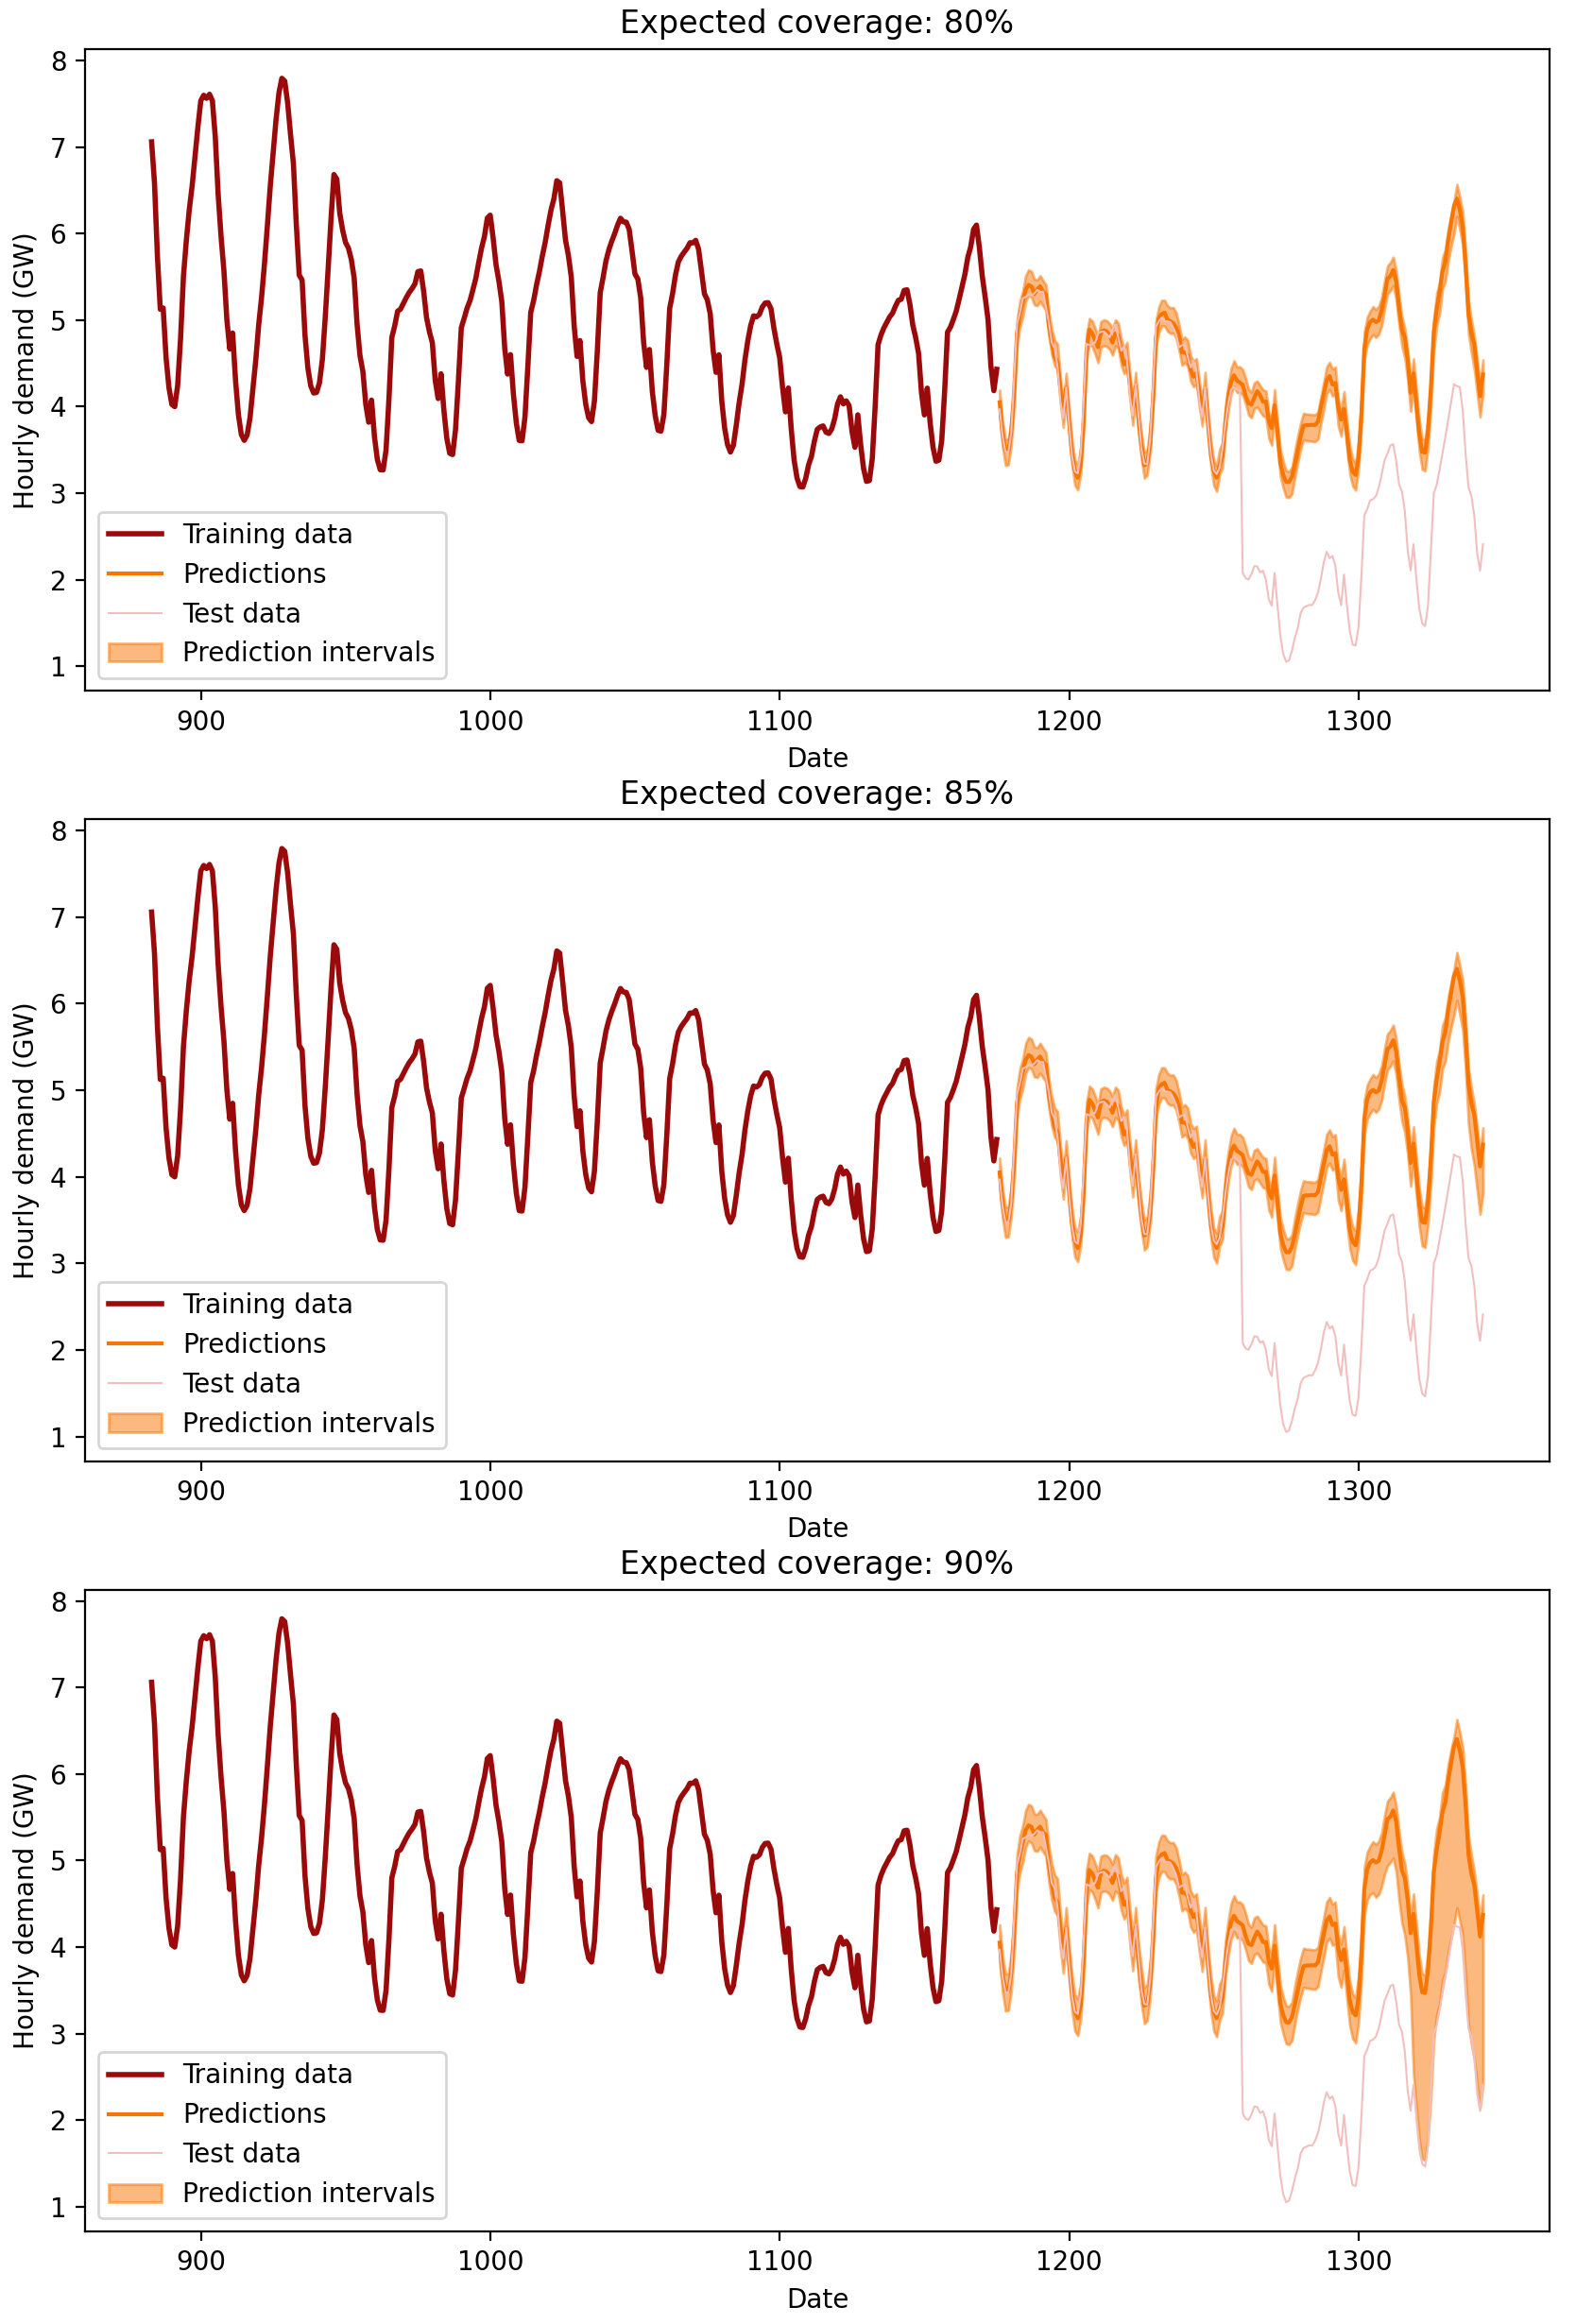
\includegraphics[width=\textwidth, height=1.25\textwidth]{Figures/timeseries/with-change-point/prediction-intervals-in-function-of-miscoverage.png}
    \caption{EnbPI with partial fit recovering intervals' width at different pace, for different $\a$ values (from top to bottom: $\a=0.20, 0.15, 0.10$).}
    \label{fig:timeseries-intervals-alpha-cpoint}
\end{figure}

These different speeds can also be noted at sub-figure \ref{subfig:timeseries-coverage-alpha-cpoint}, in which the attained global coverage for the EnbPI strategy varies non-linearly with $\a$.\\  

\begin{figure}[ht]
    \centering
    %\hspace{-10mm}
    \begin{subfigure}[b]{0.32\textwidth}
        \centering
        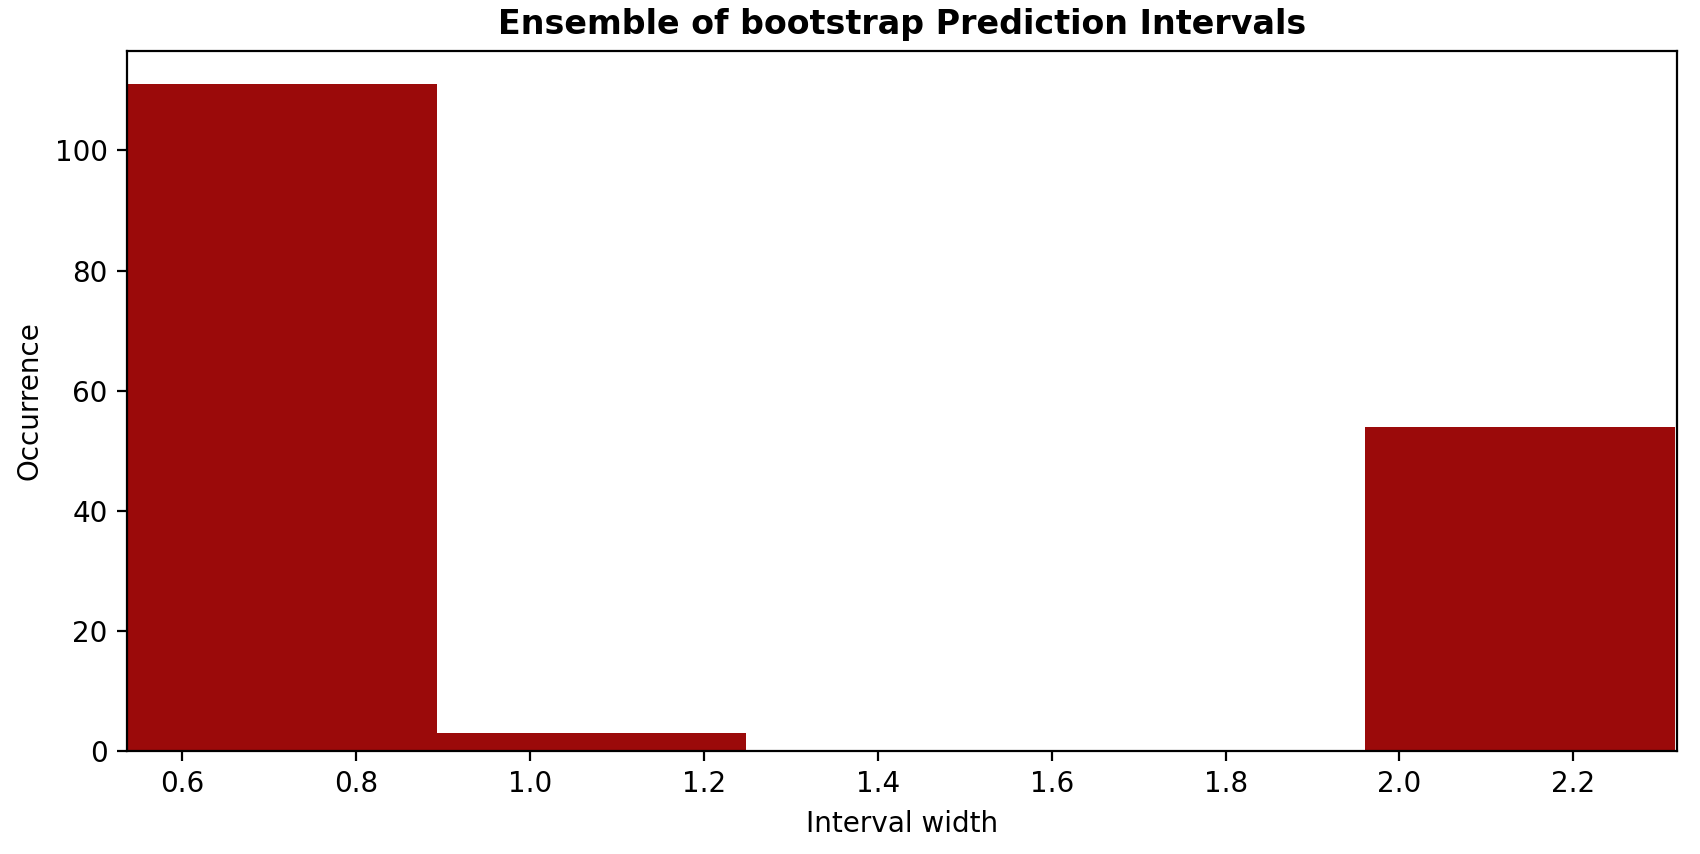
\includegraphics[width=1.05\textwidth, height=0.85\textwidth]{Figures/timeseries/with-change-point/width-occurrence-timeseries-problem-with-change-point.png}
        \caption{Intervals' width histograms}
        \label{subfig:timeseries-width-histograms-cpoint}
    \end{subfigure}
    \hfill
    \begin{subfigure}[b]{0.32\textwidth}
        \centering
        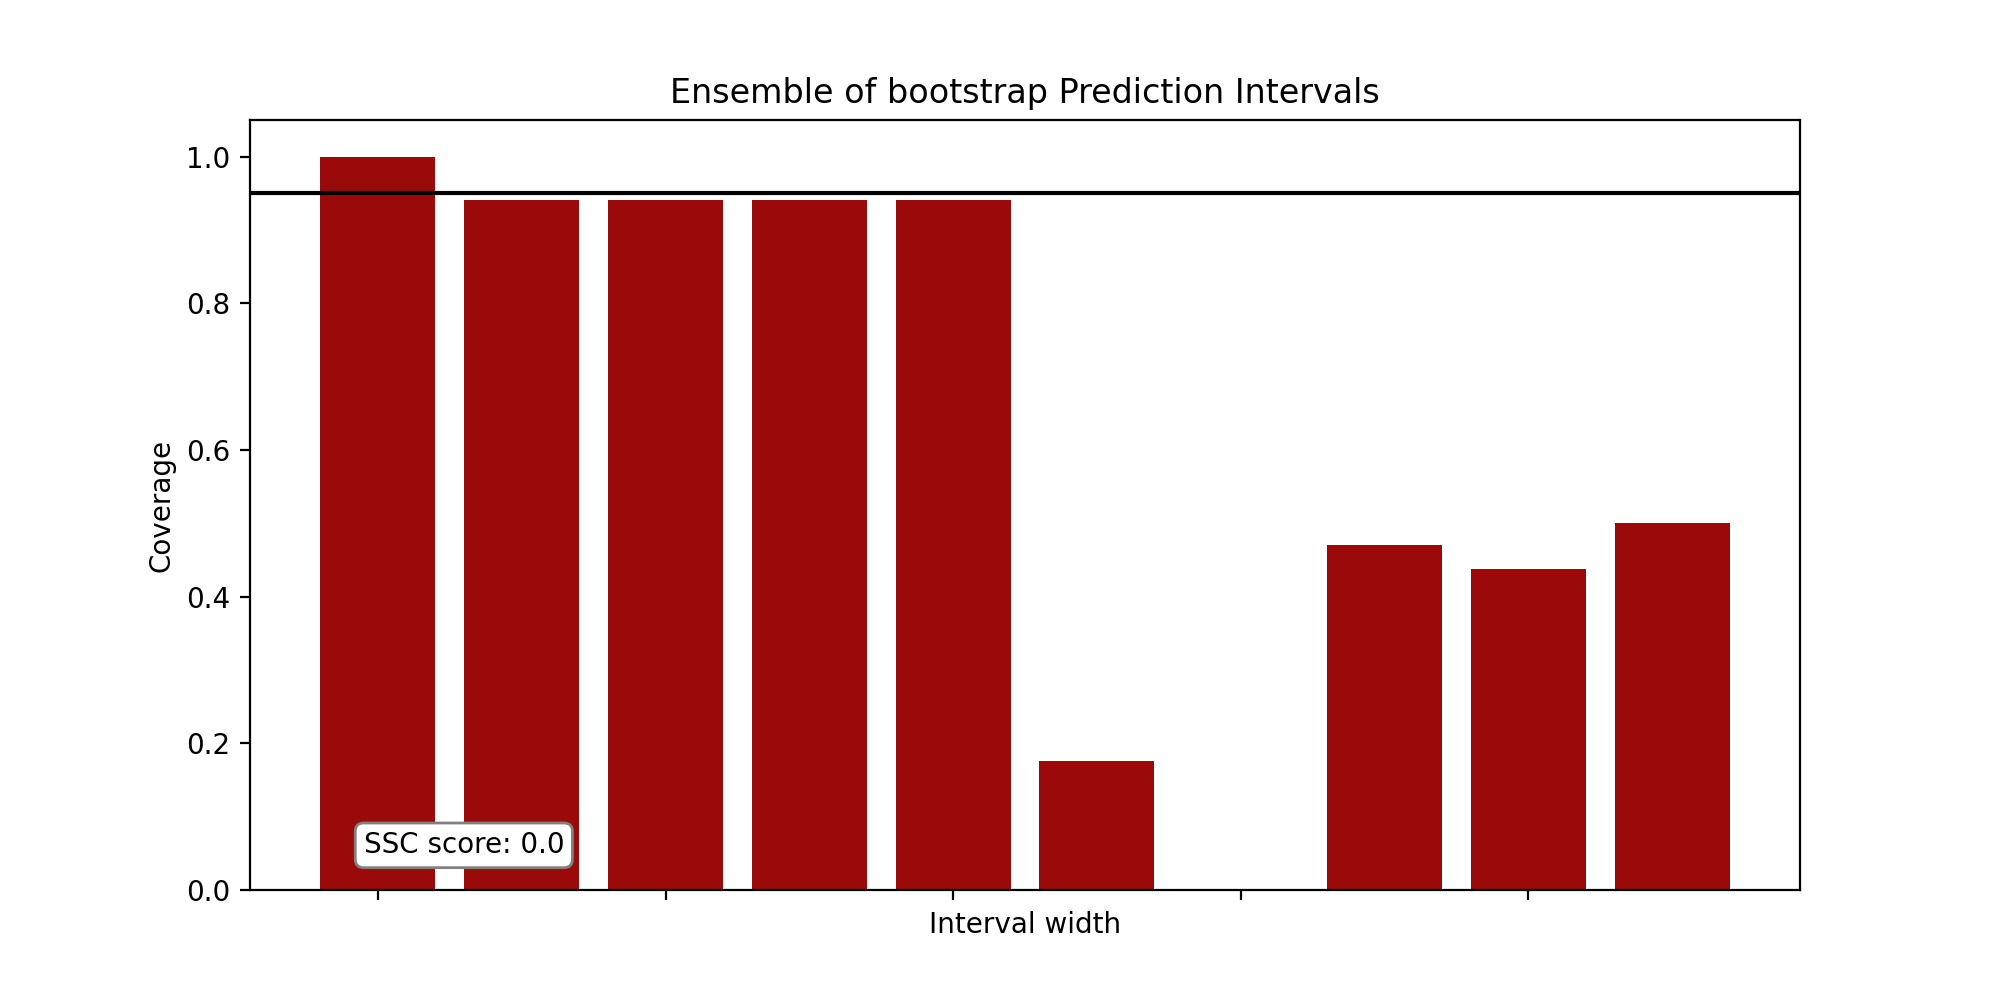
\includegraphics[width=1.15\textwidth, height=0.85\textwidth]{Figures/timeseries/with-change-point/coverage-vs-width-timeseries-problem-with-change-point.png}
        \caption{Coverage in function of intervals' width}
        \label{subfig:timeseries-coverage-width-cpoint}
    \end{subfigure}
    \hfill % adds horizontal space between figures
    \begin{subfigure}[b]{0.32\textwidth} % Adjust the width to fit your needs
        \centering
        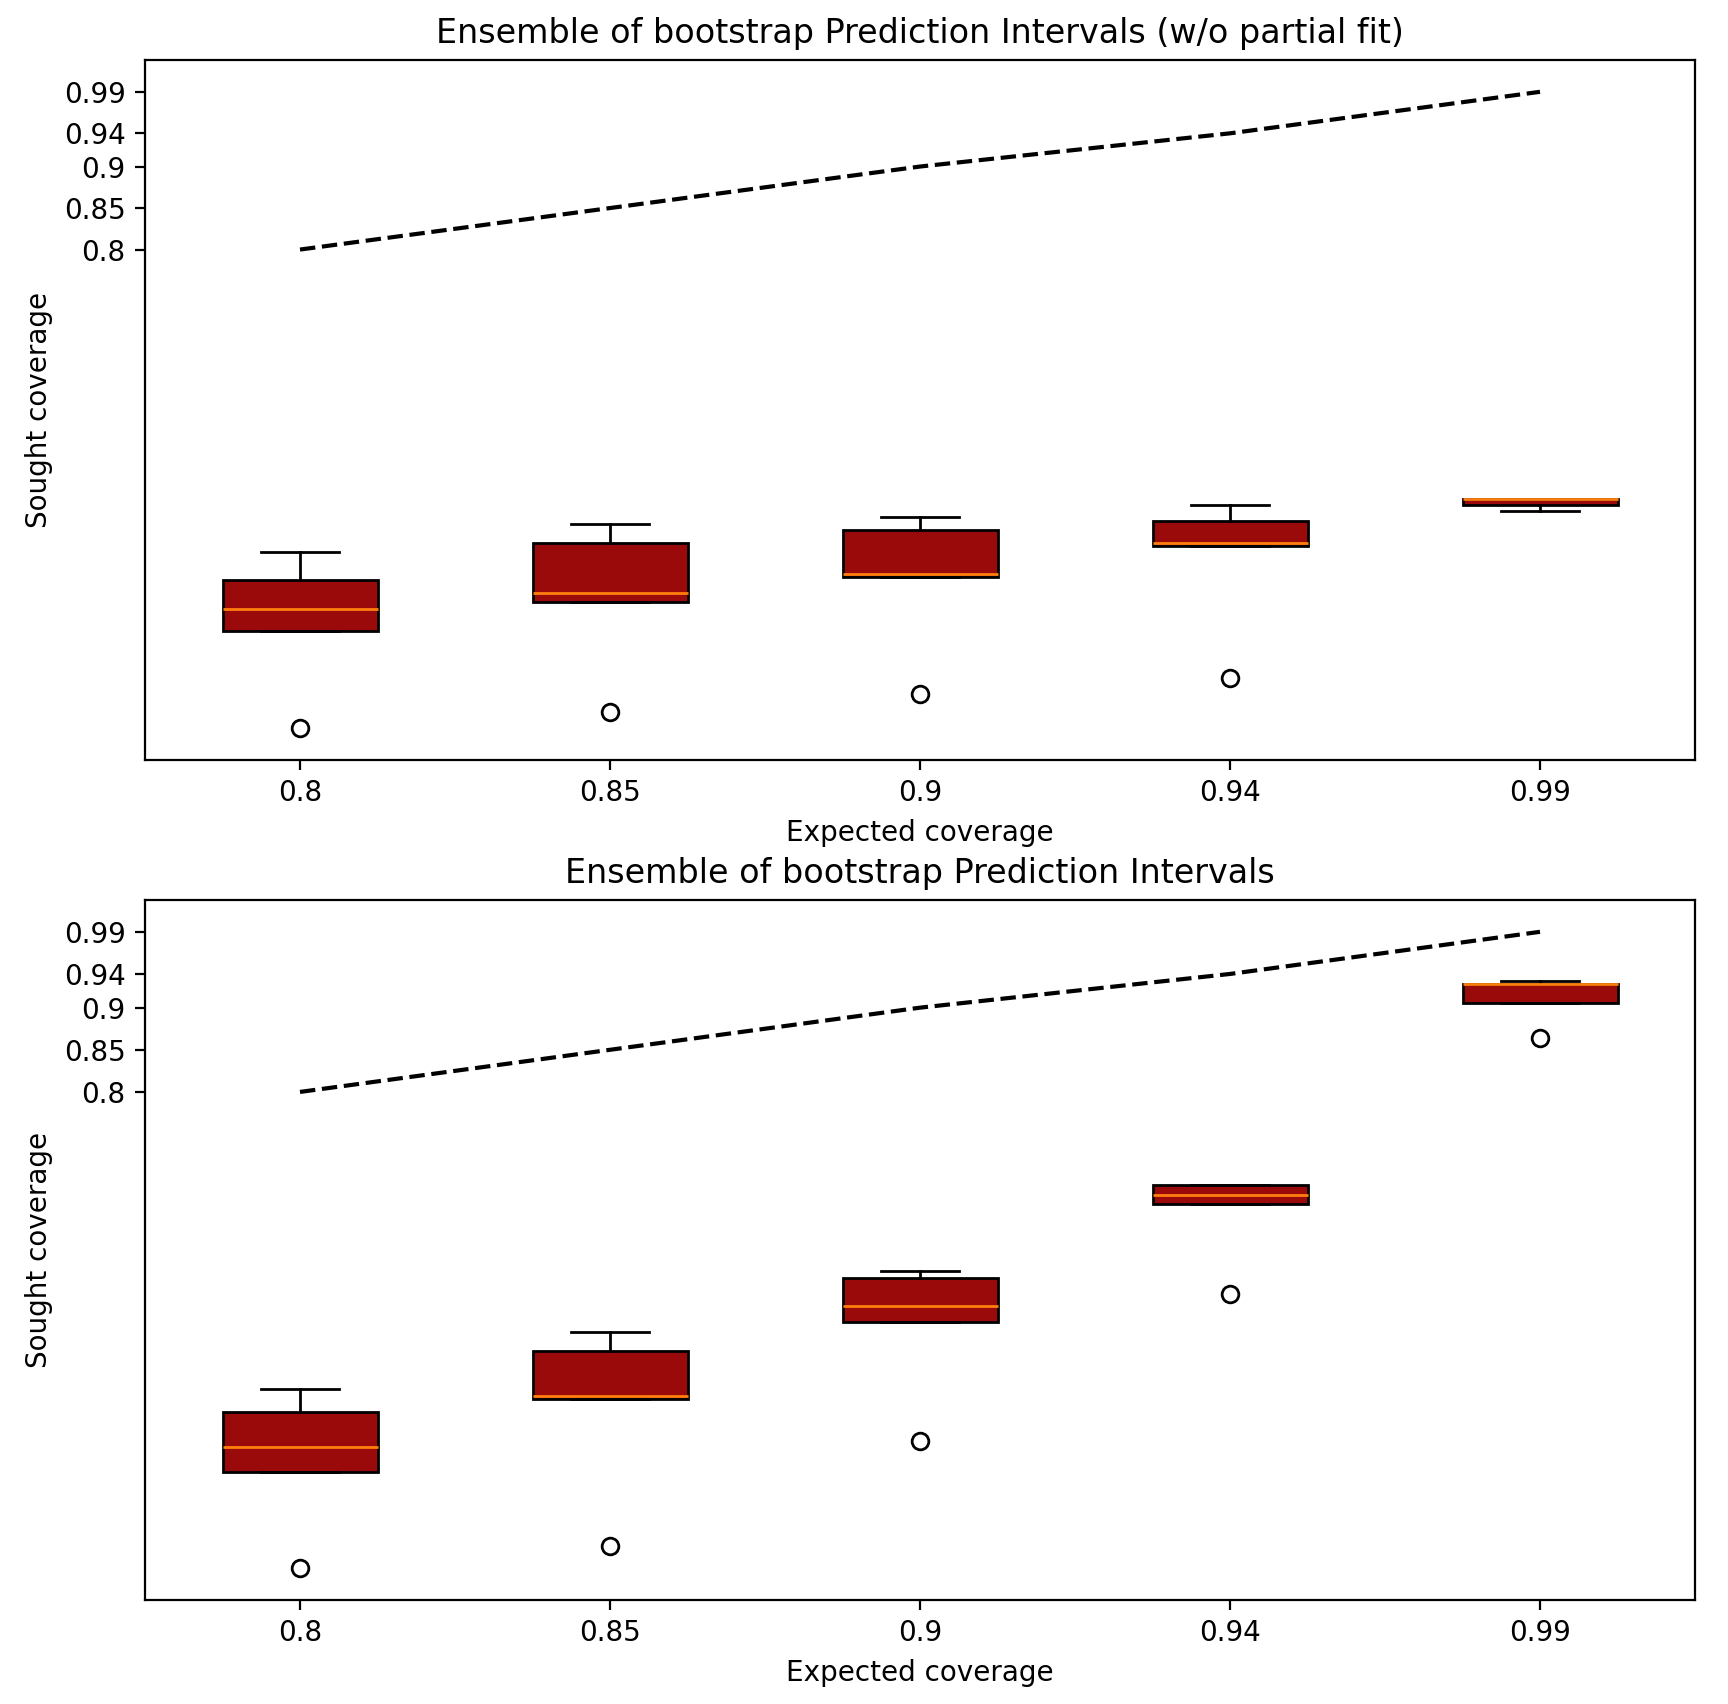
\includegraphics[width=1.15\textwidth, height=1.75\textwidth]{Figures/timeseries/with-change-point/coverage-vs-alpha-timeseries-problem-with-change-problem.png} % Adjust the filename and path
        \caption{Coverage in function of $\a$}
        \label{subfig:timeseries-coverage-alpha-cpoint}
    \end{subfigure}
    \caption{Width \& coverage distributions for the change point's (test) data ($\a=0.05$) for EnbPI. At subfigure \ref{subfig:timeseries-coverage-alpha-cpoint}, EnbPI\_{}nP \& EnbPI are displayed (top \& bottom, respectively).}
    \label{fig:timeseries-width-coverage-cpoint}
\end{figure}

Finally, while in sub-figures \ref{subfig:timeseries-width-histograms-cpoint} \& \ref{subfig:timeseries-coverage-width-cpoint} the adaptive feature of EnbPI intervals\footnote{Note the change point is also perceived with these 2 visualizations: the widest intervals correspond to those with less conditional coverage, since those were issued after the change point's recovery.} is shown; in Figure \ref{fig:timeseries-rolling-coverage-cpoint} the EnbPI's progressive coverage recovery is featured in function of time with a rolling window (while indeed EnbPI\_{}nP does not recover at all).

\begin{figure}[ht]
    \centering
    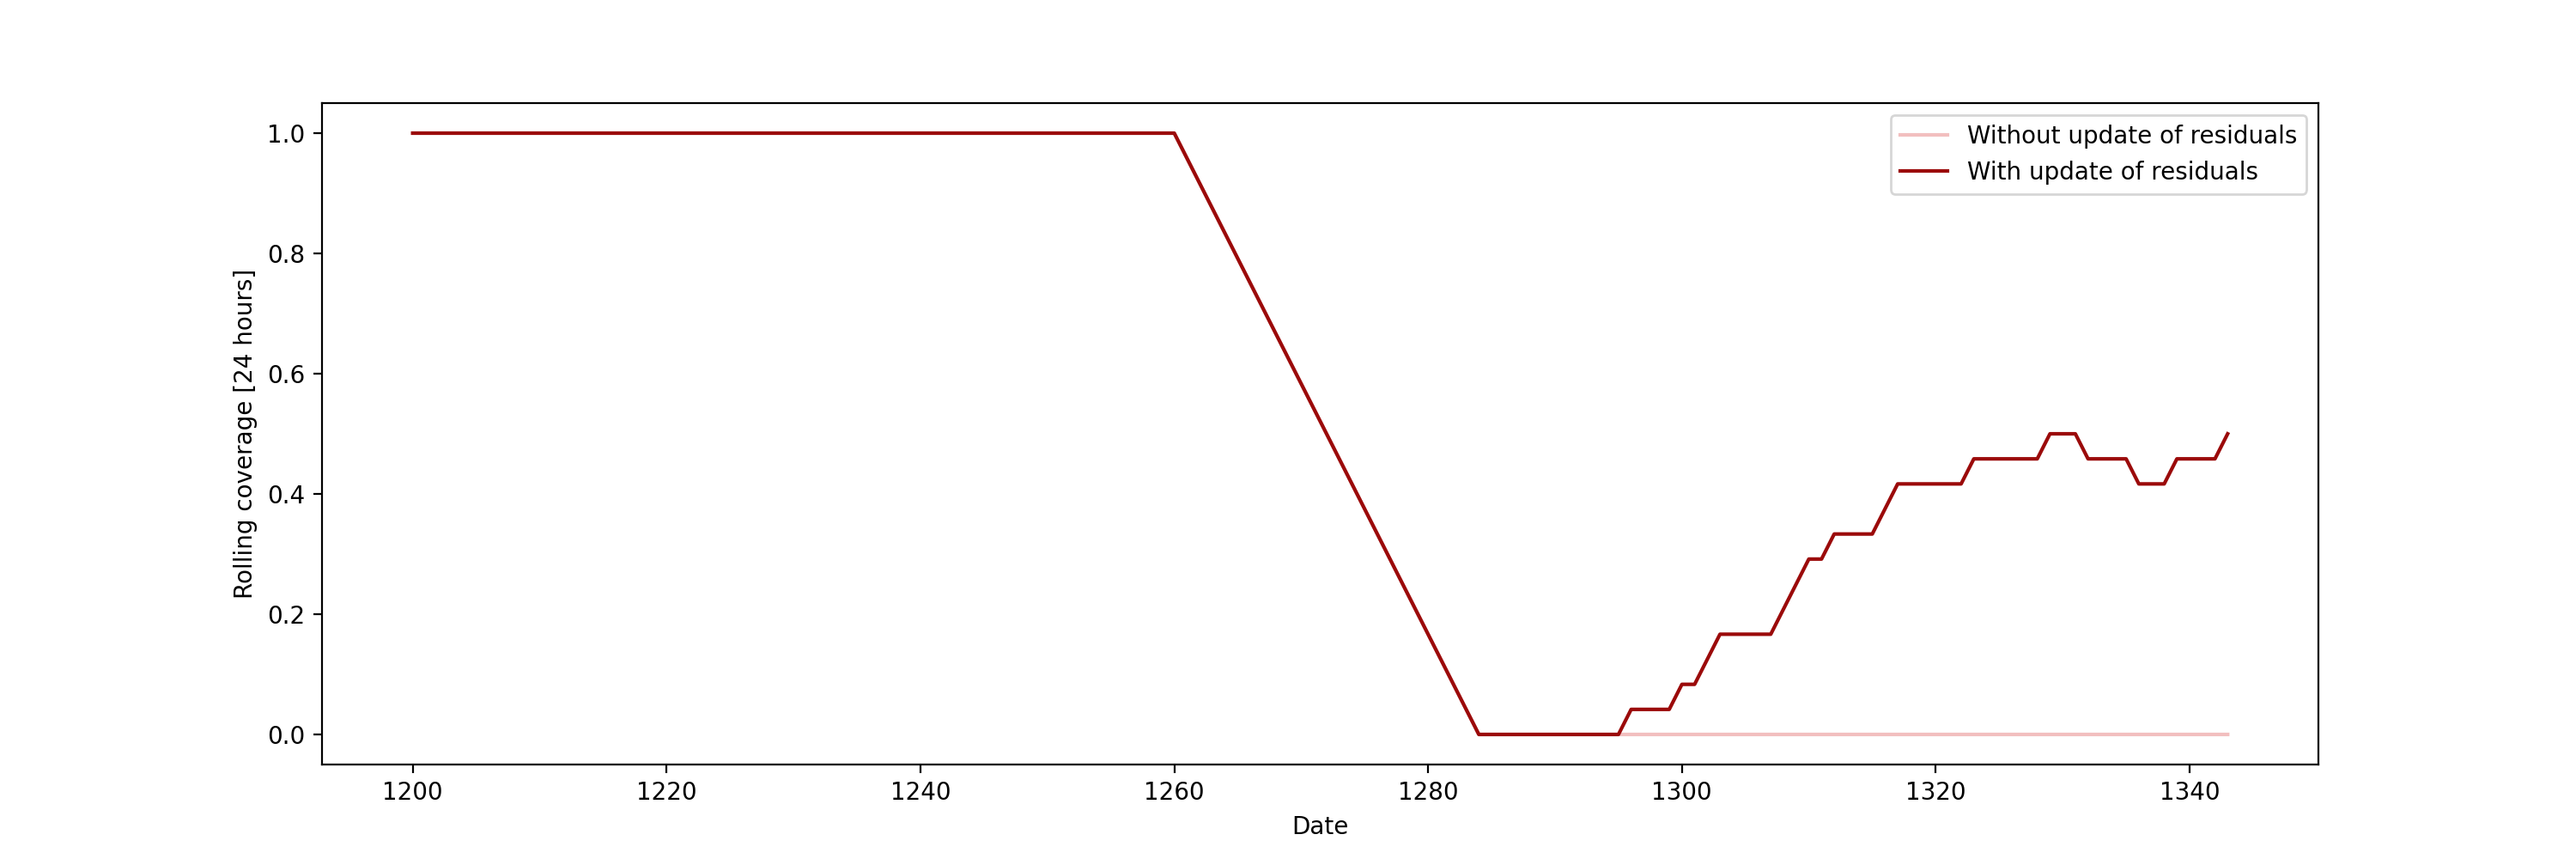
\includegraphics[width=\textwidth]{Figures/timeseries/with-change-point/rolling-coverage-with-change-point.png}
    \caption{Coverage in function of time (grouped within 24h rolling windows) for the EnbPI strategies (and change point's data).}
    \label{fig:timeseries-rolling-coverage-cpoint}
\end{figure}